\documentclass[12pt,a4paper]{report}

% ============================================================================
% PACKAGES
% ============================================================================
\usepackage[utf8]{inputenc}
\usepackage[T1]{fontenc}
\usepackage{geometry}
\usepackage{graphicx}
\usepackage{setspace}
\usepackage{fancyhdr}
\usepackage[dvipsnames]{xcolor}
\usepackage{listings}
\usepackage{enumitem}
\usepackage{tabularx}
\usepackage{longtable}
\usepackage{booktabs}
\usepackage{url}
\usepackage[most]{tcolorbox}
\usepackage{makeidx}
\usepackage{float}
\usepackage{hyperref}
\usepackage{tikz}
\usepackage{pgfplots}
\usepackage{grffile}
\pgfplotsset{compat=1.18}
\usetikzlibrary{shapes.geometric, arrows.meta, positioning, fit, backgrounds, decorations.pathreplacing, calc, shadows}

% Page Layout
\geometry{a4paper, left=1.5in, right=1in, top=1in, bottom=1in}

% Define colors
\definecolor{codegreen}{rgb}{0,0.6,0}
\definecolor{codegray}{rgb}{0.5,0.5,0.5}
\definecolor{codepurple}{rgb}{0.58,0,0.82}
\definecolor{backcolour}{rgb}{0.95,0.95,0.92}
\definecolor{darkgray}{rgb}{0.4,0.4,0.4}

% Hyperlink Setup
\hypersetup{
    colorlinks=true,
    linkcolor=blue,
    citecolor=blue,
    urlcolor=blue,
    pdftitle={PayrollX -- Smart AI-Powered Payroll Management System},
    pdfauthor={Zohaib Farhan, Fazal Abbas, Azma Munir}
}

% Code Listing Setup
\lstdefinestyle{mystyle}{
    backgroundcolor=\color{backcolour},
    basicstyle=\ttfamily\footnotesize,
    breaklines=true,
    breakatwhitespace=false,
    numbers=left,
    numberstyle=\tiny\color{codegray},
    frame=single,
    tabsize=2,
    showstringspaces=false,
    commentstyle=\color{codegreen},
    keywordstyle=\color{blue},
    stringstyle=\color{codepurple},
    captionpos=b
}
\lstset{style=mystyle}

% Define JavaScript language for listings
\lstdefinelanguage{JavaScript}{
  keywords={typeof, new, true, false, catch, function, return, null, switch, var, if, in, while, do, else, case, break, const, let, async, await, try, throw, class, export, import, default, from, of, for},
  keywordstyle=\color{blue}\bfseries,
  ndkeywords={boolean, this, Number, String, Array, Object},
  ndkeywordstyle=\color{darkgray}\bfseries,
  sensitive=true,
  comment=[l]{//},
  morecomment=[s]{/*}{*/},
  commentstyle=\color{codegreen}\ttfamily,
  stringstyle=\color{codepurple}\ttfamily,
  morestring=[b]',
  morestring=[b]",
  literate={=>}{{\textcolor{blue}{=>}}}2
}

% Lesson Learned Box
\newtcolorbox{lessonbox}[1][]{
  colback=yellow!10,
  colframe=orange!75!black,
  fonttitle=\bfseries,
  title={Lesson Learned},
  #1
}

% What Didn't Work Box
\newtcolorbox{failbox}[1][]{
  colback=red!5,
  colframe=red!75!black,
  fonttitle=\bfseries,
  title={What Didn't Work},
  #1
}

% Line Spacing
\onehalfspacing

% Index
\makeindex

\begin{document}

% ============================================================================
% TITLE PAGE 1 (GC University Format)
% ============================================================================
\begin{titlepage}
    \centering
    \vspace*{0.5cm}

    {\Large\bfseries PayrollX: A Smart AI-Powered Payroll Management System\\}
    \vspace{1.5cm}

    % GC University Logo
    
\includegraphics[width=0.35\textwidth]{gcu_logo.png}\\
    \vspace{1.5cm}

\setlength{\tabcolsep}{12pt}

\begin{tabular}{l @{\hspace{3cm}} l}
    \textbf{Submitted by} & \textbf{Zohaib Farhan} \\
    \textbf{Roll. No} & \textbf{2022-GCUL-BS-CS-GDSC-651} \\[0.3cm]
    \textbf{Submitted by} & \textbf{Fazal Abbas} \\
    \textbf{Roll. No} & \textbf{2022-GCUL-BS-CS-GDSC-670} \\[0.3cm]
    \textbf{Submitted by} & \textbf{Azma Munir} \\
    \textbf{Roll. No} & \textbf{2022-GCUL-BS-CS-GDSC-658} \\[0.4cm]
    \textbf{Session} & \textbf{2022--2026} \\[0.4cm]
    \textbf{Supervised by} & \textbf{[Supervisor Name]} \\
                           & \textbf{Assistant Professor} \\
\end{tabular}

    \vspace{1cm}

    {\Large\bfseries BS(HONS)\\}
    {\Large IN\\}
    {\Large\bfseries COMPUTER SCIENCE\\}

    \vfill

    \vspace{0.3cm}
    {\Large\bfseries DEPARTMENT OF COMPUTER SCIENCE\\}
    {\Large\bfseries GC UNIVERSITY LAHORE\\}
\end{titlepage}

% ============================================================================
% TITLE PAGE 2 (Submission Statement)
% ============================================================================
\begin{titlepage}
    \centering
    \vspace*{1cm}

    {\Large\bfseries PayrollX: A Smart AI-Powered Payroll Management System\\}
    \vspace{1cm}

    {\large Submitted to GC University Lahore in partial fulfillment\\
    of the requirements for the award of degree of\\}
    \vspace{1.5cm}

    {\Large\bfseries BS(HONS)\\}
    \vspace{0.3cm}
    {\Large IN\\}
    \vspace{0.3cm}
    {\Large\bfseries COMPUTER SCIENCE\\}

    \vspace{1.5cm}

    \begin{tabular}{ll}
        \textbf{Submitted by} & Zohaib Farhan \\
        \textbf{Roll. No}     & 2022-GCUL-BS-CS-GDSC-651 \\[0.3cm]
        \textbf{Submitted by} & Fazal Abbas \\
        \textbf{Roll. No}     & 2022-GCUL-BS-CS-GDSC-670 \\[0.3cm]
        \textbf{Submitted by} & Azma Munir \\
        \textbf{Roll. No}     & 2022-GCUL-BS-CS-GDSC-658 \\[0.4cm]
        \textbf{Session}      & 2022 -- 2026 \\[0.4cm]
        \textbf{Supervised by}& {[}Supervisor Name{]} \\
                              & Assistant Professor \\
    \end{tabular}

    \vfill

    {\Large\bfseries DEPARTMENT OF COMPUTER SCIENCE\\}
    \vspace{0.3cm}
    {\Large\bfseries GC UNIVERSITY LAHORE\\}
\end{titlepage}

% ============================================================================
% FRONT MATTER (Roman Numerals)
% ============================================================================
\pagenumbering{roman}

% ----------------------------------------------------------------------------
% DECLARATION
% ----------------------------------------------------------------------------
\chapter*{Declaration}
\addcontentsline{toc}{chapter}{Declaration}

We, \textbf{Zohaib Farhan} (Roll No. 2022-GCUL-BS-CS-GDSC-651), \textbf{Fazal Abbas} (Roll No. 2022-GCUL-BS-CS-GDSC-670), and \textbf{Azma Munir} (Roll No. 2022-GCUL-BS-CS-GDSC-658), students of \textbf{BS(Hons)} in the subject of \textbf{Computer Science}, session \textbf{2022--2026}, hereby declare that the matter printed in this project titled \textbf{``PayrollX: A Smart AI-Powered Payroll Management System''} is our own work and has not been printed, published, or submitted as a research work, thesis, or publication in any form in any University, Research Institution, or similar body in Pakistan or abroad.

We further declare that every line of code, every design decision, and every implementation detail presented in this document represents our original work, completed under proper academic supervision. This project was built from scratch and was not downloaded or copied from any external source.

\vspace{3cm}

\noindent\textbf{Date:} \rule{3cm}{0.4pt} \hfill \textbf{Signatures of Deponents}

\vspace{1cm}
\noindent\hfill Zohaib Farhan (2022-GCUL-BS-CS-GDSC-651) \rule{4cm}{0.4pt}

\vspace{0.5cm}
\noindent\hfill Fazal Abbas (2022-GCUL-BS-CS-GDSC-670) \rule{4cm}{0.4pt}

\vspace{0.5cm}
\noindent\hfill Azma Munir (2022-GCUL-BS-CS-GDSC-658) \rule{4cm}{0.4pt}

% ----------------------------------------------------------------------------
% RESEARCH COMPLETION CERTIFICATE
% ----------------------------------------------------------------------------
\chapter*{Research Completion Certificate}
\addcontentsline{toc}{chapter}{Research Completion Certificate}

It is certified that the research work contained in this project titled \textbf{``PayrollX: A Smart AI-Powered Payroll Management System''} has been carried out by \textbf{Zohaib Farhan} (Roll No. 2022-GCUL-BS-CS-GDSC-651), \textbf{Fazal Abbas} (Roll No. 2022-GCUL-BS-CS-GDSC-670), and \textbf{Azma Munir} (Roll No. 2022-GCUL-BS-CS-GDSC-658) under my supervision.

\vspace{3cm}

\hfill\rule{5cm}{0.4pt}

\hfill\textbf{Supervisor Name}

\hfill Designation

\vspace{2cm}

\noindent\textbf{Date:} \rule{3cm}{0.4pt}

\vspace{2cm}

\noindent\textbf{Submitted Through}

\vspace{2cm}

\noindent\rule{5cm}{0.4pt} \hfill \rule{5cm}{0.4pt}

\noindent\textbf{Dr. Syed Asad Raza Kazmi} \hfill \textbf{Controller of Examination}

\noindent\textbf{Director} \hfill GC University Lahore

\noindent Department of Computer Science

\noindent GC University Lahore

% ----------------------------------------------------------------------------
% ACKNOWLEDGEMENTS
% ----------------------------------------------------------------------------
\chapter*{Acknowledgements}
\addcontentsline{toc}{chapter}{Acknowledgements}

First and foremost, all praise to Allah, who gave us the strength to persist through long debugging sessions and the patience to navigate the complexities of building a production-quality payroll system as students.

We want to thank our supervisor, who challenged us to go beyond a simple CRUD application and incorporate AI-driven analytics into PayrollX. Their guidance on system design, Pakistani tax compliance, and project scope kept us focused and productive throughout the development cycle.

A sincere thank you to the open-source community. The developers behind Express.js, PostgreSQL, React, Tailwind CSS, shadcn/ui, and TanStack Query built the foundations that made this project possible. We stand on the shoulders of giants.

To the GC University faculty who taught us software engineering principles, database design, and web technologies: this project is the direct application of four years of learning. Every concept --- from database normalisation to JWT authentication to component-based UI development --- found its place in this codebase.

To our families: thank you for tolerating the late nights, the missed dinners, and the incomprehensible technical discussions at the dinner table. Your encouragement meant everything.

And to every student in Pakistan struggling to bridge the gap between classroom theory and real-world software development --- PayrollX is proof that it can be done.

% ----------------------------------------------------------------------------
% DEDICATION
% ----------------------------------------------------------------------------
\chapter*{Dedication}
\addcontentsline{toc}{chapter}{Dedication}

\vspace*{3cm}
\begin{center}
\textit{To our families, whose sacrifices made our education possible.\\
To our teachers, who gave us the knowledge and the confidence to build.\\
To every small business in Pakistan still running payroll on spreadsheets ---\\
we built this for you.}
\end{center}

% ----------------------------------------------------------------------------
% ABSTRACT
% ----------------------------------------------------------------------------
\chapter*{Abstract}
\addcontentsline{toc}{chapter}{Abstract}

Payroll and human resource management in Pakistani small and medium-sized enterprises remain largely manual, error-prone, and non-compliant with Federal Board of Revenue (FBR) tax regulations. Organisations relying on spreadsheets and paper-based processes face recurring problems: incorrect salary calculations, delayed payslip distribution, inconsistent leave tracking, and an absence of actionable HR analytics.

We developed \textbf{PayrollX}, a Smart AI-Powered Payroll Management System, to address these challenges. PayrollX is a full-stack web application consisting of a Node.js/Express.js backend connected to a PostgreSQL relational database, and a React/TypeScript frontend built with Vite and shadcn/ui. The system provides role-based dashboards for HR administrators and employees, automating the complete payroll cycle from attendance recording through to payslip generation, while enforcing compliance with FBR tax slabs (2024--25), EOBI, and SESSI contribution rules.

Beyond core payroll automation, PayrollX incorporates five AI-driven modules: fraud detection (identifying duplicate bank accounts, ghost employees, and salary spikes), salary anomaly detection (statistical outlier analysis across departments), payroll forecasting (time-series trend analysis for budget planning), salary recommendations (market comparison and internal equity analysis), and an HR chatbot (intent-based natural language queries for leave balances, salary information, and attendance).

The system was evaluated against all defined functional requirements. All six primary objectives were achieved, including automated payroll processing for up to 200 employees, FBR-compliant tax calculations, real-time in-app notifications, and a self-service employee portal. The test suite comprises 107 tests across backend (Jest) and frontend (Vitest) layers, with all tests passing.

\textbf{Keywords:} Payroll Management, Human Resources, AI-Powered Analytics, FBR Tax Compliance, React, Node.js, PostgreSQL, Pakistan

% ----------------------------------------------------------------------------
% TABLE OF CONTENTS
% ----------------------------------------------------------------------------
\tableofcontents

% ----------------------------------------------------------------------------
% LIST OF TABLES
% ----------------------------------------------------------------------------
\listoftables
\addcontentsline{toc}{chapter}{List of Tables}

% ----------------------------------------------------------------------------
% LIST OF FIGURES
% ----------------------------------------------------------------------------
\listoffigures
\addcontentsline{toc}{chapter}{List of Figures}

% ============================================================================
% MAIN CONTENT (Arabic Numerals)
% ============================================================================
\pagenumbering{arabic}

% Header and Footer for main content
\pagestyle{fancy}
\fancyhf{}
\fancyhead[L]{\leftmark}
\fancyhead[R]{\thepage}
\renewcommand{\headrulewidth}{0.4pt}

% ============================================================================
% CHAPTER 1: INTRODUCTION
% ============================================================================
\chapter{Introduction}
\label{chap:introduction}

\section{Background and Motivation}

Payroll management is one of the most critical and legally sensitive functions of any organisation. In Pakistan, the challenge is compounded by a regulatory framework that requires employers to comply with Federal Board of Revenue (FBR) income tax slabs, Employees' Old-Age Benefits Institution (EOBI) contributions, and the Sindh Employees' Social Security Institution (SESSI) scheme. Despite these requirements, the majority of small and medium-sized enterprises (SMEs) in Pakistan continue to process payroll manually using spreadsheets or basic accounting software that lacks statutory compliance features \cite{WorldBank2022}.

The consequences of manual payroll processing are well-documented: salary calculation errors occur in up to 33\% of manually-processed payrolls \cite{APA2023}; delayed payslip distribution creates employee dissatisfaction; leave balance discrepancies lead to disputes; and the absence of audit trails makes compliance verification difficult. For an organisation of even fifty employees, manual payroll processing can consume an entire working week each month.

Beyond the operational burden, manual processes create data silos. Attendance records, leave applications, and salary information are stored in separate files or registers with no shared reference, making it impossible to generate meaningful HR analytics. HR managers cannot easily answer questions such as: which department has the highest absenteeism rate, which employees are approaching their leave entitlement limits, or what is the projected payroll cost for the next quarter.

This project was motivated by the observed gap between the availability of modern HR technology and its adoption by Pakistani SMEs. Enterprise systems such as SAP HCM and Oracle PeopleSoft exist but are prohibitively expensive and complex. Cloud-based alternatives such as Gusto and BambooHR are designed for Western markets and do not support Pakistani tax structures. The result is that Pakistani businesses are left without a suitable, affordable, compliant payroll solution.

\section{Project Overview}

We developed \textbf{PayrollX}, a comprehensive, AI-powered payroll management system designed for Pakistani organisations. PayrollX integrates seven core HR functions into a single web application:

\begin{itemize}
    \item \textbf{Employee Management:} Complete employee records including personal information, department, designation, salary structure, and bank account details.
    \item \textbf{Attendance Tracking:} Daily check-in/check-out recording with manual HR override capability.
    \item \textbf{Leave Management:} Multi-type leave requests, HR approval workflows, and automatic balance deduction.
    \item \textbf{Payroll Processing:} Automated salary computation with FBR-compliant tax deductions, EOBI, and SESSI contributions, resulting in per-employee payslips.
    \item \textbf{AI Analytics:} Five AI-driven modules providing fraud detection, anomaly detection, payroll forecasting, salary recommendations, and an HR chatbot.
    \item \textbf{Notifications:} Real-time in-app notifications for key HR events.
    \item \textbf{Settings and Compliance:} Configurable public holidays, tax tables, and system preferences.
\end{itemize}

The system is built as a two-application architecture: a Node.js/Express.js backend with PostgreSQL, and a React/TypeScript frontend. Role-based access control ensures HR administrators and employees see only the features and data appropriate to their role.

\section{Objectives}

We established the following objectives for PayrollX:

\textbf{Primary Objectives:}
\begin{enumerate}
    \item Build a secure, role-based web application supporting HR administrators and employees.
    \item Automate payroll calculation with FBR 2024--25 tax slab compliance, EOBI, and SESSI deductions.
    \item Provide a centralised attendance and leave management module with automatic balance tracking.
    \item Implement an event-driven in-app notification system for key HR events.
    \item Deliver a self-service employee portal for profile management, leave requests, and payslip access.
    \item Integrate AI-driven analytics for fraud detection, salary anomaly detection, payroll forecasting, salary recommendations, and conversational HR queries.
\end{enumerate}

\textbf{Secondary Objectives:}
\begin{enumerate}
    \item Achieve payroll computation for 200 employees within 10 seconds.
    \item Ensure API responses for standard operations complete within 500\,ms.
    \item Maintain a comprehensive test suite with unit tests for all backend services.
    \item Design the system for extensibility, allowing future integration of biometric systems and real ML models.
\end{enumerate}

\section{Scope}

\textbf{In Scope:}
\begin{itemize}
    \item Employee management (CRUD) with department and salary structure assignment
    \item Daily attendance check-in/check-out and manual HR marking
    \item Leave request submission, approval/rejection workflow, and balance tracking
    \item Monthly payroll runs with FBR tax slab calculation, EOBI (0.75\%), and SESSI (0.75\% up to PKR~25,000 wages) deductions
    \item Per-employee payslip generation and download
    \item AI-based fraud detection, salary anomaly detection, payroll forecasting, salary recommendations, and HR chatbot
    \item Role-based dashboards for HR administrators and employees
    \item In-app notifications for leave status changes and salary credits
    \item System settings including public holiday management and tax configuration
\end{itemize}

\textbf{Out of Scope:}
\begin{itemize}
    \item Biometric or physical access-control integration
    \item Email or SMS notification delivery
    \item Mobile native application
    \item Multi-tenancy (multiple organisations sharing a single deployment)
    \item Real-time salary market data integration (simulated data used for recommendations)
    \item CI/CD pipeline integration or containerised deployment
\end{itemize}

\begin{lessonbox}
Scope discipline saved this project. Early in development we discussed adding biometric integration, email notifications, and a mobile app in the same semester. Our supervisor correctly pointed out that delivering a polished, complete core system would be more valuable than delivering many half-finished features. The discipline to say ``no'' to out-of-scope requests is one of the most important skills we learned.
\end{lessonbox}

\section{Document Organization}

This document is organised into seven chapters. Chapter~2 presents a literature review of existing HR and payroll systems, academic research, and the identified gap. Chapter~3 covers the methodology including requirements analysis, development approach, and system design. Chapter~4 details the implementation of all system components with code listings and interface screenshots. Chapter~5 presents testing results and evaluation against defined requirements. Chapter~6 concludes the project with lessons learned and future directions. Chapter~7 lists all references cited in this document.

% ============================================================================
% CHAPTER 2: LITERATURE REVIEW
% ============================================================================
\chapter{Literature Review}
\label{chap:literature}

Before writing any code, we conducted a comprehensive review of existing payroll and HR management systems, relevant academic literature, and the Pakistani regulatory context. This chapter summarises our findings and establishes the gap that motivated PayrollX.

\section{Evolution of Payroll and HR Systems}

Payroll management has evolved through four distinct generations of technology. In the 1970s and 1980s, mainframe-based payroll systems handled large enterprise payrolls but required dedicated IT infrastructure and trained operators. The 1990s brought PC-based accounting packages, making payroll accessible to smaller organisations, though these systems were siloed from HR functions.

The 2000s saw the rise of Enterprise Resource Planning (ERP) systems that integrated HR, payroll, and finance. SAP HCM and Oracle PeopleSoft became the dominant platforms for large enterprises, offering comprehensive functionality but at a cost and complexity that placed them out of reach for SMEs \cite{BenAri2008}. Research by Dessler (2020) highlights that self-service HR portals significantly reduce administrative burden by enabling employees to handle routine tasks such as leave applications independently.

The current era is defined by cloud-based HR Software-as-a-Service (SaaS) platforms. Products such as Gusto, BambooHR, and ADP Workforce Now offer integrated payroll, benefits, and HR management through subscription models. However, these platforms are built for Western regulatory frameworks (US, UK, EU) and do not natively support Pakistani tax structures, EOBI contributions, or SESSI requirements.

\section{Existing Systems and Tools}

Table~\ref{tab:tool_comparison} summarises the key HR and payroll systems we evaluated during our literature review.

\begin{table}[H]
\centering
\caption{Comparison of Existing HR and Payroll Systems}
\label{tab:tool_comparison}
\begin{tabular}{|l|l|l|l|}
\hline
\textbf{System} & \textbf{Type} & \textbf{Pakistan Tax} & \textbf{Cost} \\
\hline
SAP HCM         & Enterprise ERP    & No (custom config) & \$100,000+/year \\
\hline
Oracle PeopleSoft & Enterprise ERP  & No (custom config) & \$80,000+/year \\
\hline
Gusto           & Cloud SaaS        & No (US only)       & \$40/month + per employee \\
\hline
BambooHR        & Cloud SaaS        & No (US only)       & \$6--\$9/employee/month \\
\hline
ADP Workforce   & Cloud SaaS        & No (US/UK)         & Custom pricing \\
\hline
QuickBooks Payroll & Desktop/Cloud  & No (US/Canada)     & \$45+/month \\
\hline
PayrollX        & Web Application   & Yes (FBR 2024--25) & Free (open source) \\
\hline
\end{tabular}
\end{table}

\subsection{Analysis of Enterprise Solutions}

SAP HCM and Oracle PeopleSoft provide comprehensive HR and payroll functionality but are designed for large enterprises with dedicated IT teams. Their complexity, cost, and implementation timelines (typically six to twelve months) make them impractical for Pakistani SMEs. Customising them for FBR compliance requires expensive consulting engagements.

\subsection{Analysis of Cloud SaaS Platforms}

Cloud-based platforms such as Gusto and BambooHR represent a significant usability improvement over legacy ERP systems. However, they are fundamentally designed for the US market. Their payroll engines compute federal and state income tax, Social Security, and Medicare contributions --- none of which apply in Pakistan. While API-based customisation is theoretically possible, adapting these platforms for FBR tax slabs, EOBI, and SESSI would require significant development effort and ongoing maintenance as tax regulations change.

Furthermore, these platforms charge per-employee fees that, while affordable in USD, become significant in PKR for organisations of 50--200 employees, which is the typical size of Pakistani SME that most needs a digital payroll solution.

\section{Pakistani Regulatory Context}

The Pakistani payroll context has specific statutory requirements that any compliant system must address:

\textbf{FBR Income Tax (Tax Year 2024--25):} The Federal Board of Revenue publishes annual income tax slabs. For tax year 2024--25, salaried employees who are tax filers enjoy progressive rates ranging from 0\% (annual income up to PKR~600,000) to 35\% (annual income above PKR~4,100,000). Non-filers pay approximately 10\% higher rates. Any payroll system for Pakistan must implement these slabs correctly and apply the filer/non-filer distinction.

\textbf{EOBI:} The Employees' Old-Age Benefits Institution requires a 0.75\% employer contribution on all employee wages. This is a mandatory statutory deduction that must be computed and reported monthly.

\textbf{SESSI:} The Sindh Employees' Social Security Institution requires a 0.75\% employer contribution on wages up to PKR~25,000. This applies to employees covered under the provincial social security scheme.

Existing commercial software does not implement these Pakistan-specific rules, leaving Pakistani organisations to either manually compute deductions or rely on non-compliant calculations.

\section{Related Academic Research}

Several academic works informed our design:

Automatic payroll systems have been shown to reduce payroll processing errors by up to 80\% compared to manual methods \cite{scribd}. Studies on HR information systems in developing countries consistently find that the primary barriers to adoption are cost, complexity, and lack of localisation --- precisely the gaps PayrollX addresses.

Research on rule-based anomaly detection in financial systems \cite{AccountingReview2021} demonstrates that simple statistical methods (Z-score analysis, threshold-based rules) achieve high precision for detecting outliers in structured financial datasets such as payroll records. This finding supported our decision to implement AI features using explainable rule-based algorithms rather than opaque machine learning models --- an important consideration for an HR system where decisions must be auditable.

The HR chatbot literature shows that intent-based classification systems achieve sufficient accuracy for the narrow domain of HR queries (leave balances, salary enquiries, attendance status) without requiring large language model infrastructure \cite{Adamopoulou2020}. This guided our chatbot design toward a rule-based intent classifier rather than an LLM-based solution.

\section{Identified Gap}

Our literature review revealed a clear and actionable gap in the HR software landscape for Pakistani organisations:

\begin{itemize}
    \item Enterprise ERP systems are powerful but prohibitively expensive and complex for SMEs
    \item Cloud SaaS platforms offer good usability but lack Pakistani tax compliance features
    \item No existing open-source solution provides FBR-compliant payroll with integrated AI analytics
    \item The combination of payroll automation, AI-driven insights, and Pakistani statutory compliance in a single affordable platform does not currently exist
\end{itemize}

This gap defined PayrollX's value proposition: an open-source, full-featured, FBR-compliant payroll management system with AI-driven HR analytics, built specifically for the Pakistani market.

\begin{failbox}
We initially evaluated building PayrollX on top of an existing open-source payroll library. After two weeks of investigation, we found that available libraries (mostly Node-payroll and similar packages) assumed US tax rules at a fundamental level and could not be adapted for FBR compliance without rewriting the core computation engine. We decided to build the tax calculator from scratch, which ultimately gave us complete control over the computation logic and made FBR compliance straightforward.
\end{failbox}

% ============================================================================
% CHAPTER 3: METHODOLOGY
% ============================================================================
\chapter{Methodology}
\label{chap:methodology}

This chapter describes the development methodology, requirements analysis, and system design decisions that shaped PayrollX.

\section{Development Approach}

We followed an \textbf{Agile} development methodology with two-week sprints. This approach was chosen because:

\begin{itemize}
    \item HR system requirements are well-understood but the correct design of individual modules (particularly the payroll computation engine) requires iteration
    \item Iterative delivery enabled our supervisor to review working increments and provide feedback before the next module was built
    \item Agile's emphasis on working software over comprehensive documentation suited our student timeline while still producing a production-quality system
    \item The modular nature of HR functionality (attendance, leave, payroll, AI) mapped naturally to sprint boundaries
\end{itemize}

\textbf{Sprint Structure:}
\begin{itemize}
    \item Sprint 1--2: Project scaffolding, database schema (18 migrations), JWT authentication
    \item Sprint 3--4: Employee management, department management, salary structures
    \item Sprint 5--6: Attendance management, leave management, leave balance tracking
    \item Sprint 7--8: Payroll computation engine, payslip generation, FBR tax calculator
    \item Sprint 9--10: AI modules (fraud detection, anomaly detection, forecasting, recommendations, chatbot)
    \item Sprint 11--12: Frontend dashboards, notifications, settings, testing, and documentation
\end{itemize}

\section{Requirements Analysis}

Requirements were gathered through analysis of existing HR systems, the Pakistani regulatory framework, and consultation with our supervisor. Requirements are documented using the MoSCoW prioritisation method and organised by module.

\subsection{Functional Requirements}

\subsubsection{Authentication and Authorisation}

\begin{table}[H]
\centering
\caption{Authentication and Authorisation Requirements}
\label{tab:auth_req}
\begin{tabular}{|p{2.2cm}|p{5cm}|p{5cm}|}
\hline
\textbf{ID} & \textbf{Requirement} & \textbf{Acceptance Criteria} \\
\hline
FR-AUTH-01 & Users shall log in with email and password & Email validation, bcrypt password comparison \\
\hline
FR-AUTH-02 & System shall issue JWT access and refresh tokens & Access token 15 min, refresh token 7 days with rotation \\
\hline
FR-AUTH-03 & System shall support three roles: admin, hr, employee & Role stored in JWT payload, enforced server-side \\
\hline
FR-AUTH-04 & System shall restrict HR-only endpoints to HR/admin roles & 403 Forbidden returned for unauthorised role \\
\hline
FR-AUTH-05 & System shall allow authenticated users to log out & Refresh token invalidated in database on logout \\
\hline
FR-AUTH-06 & System shall return generic error on invalid credentials & No field-level disclosure of email or password error \\
\hline
\end{tabular}
\end{table}

\subsubsection{Employee Management}

\begin{table}[H]
\centering
\caption{Employee Management Requirements}
\label{tab:emp_req}
\begin{tabular}{|p{2.2cm}|p{5cm}|p{5cm}|}
\hline
\textbf{ID} & \textbf{Requirement} & \textbf{Acceptance Criteria} \\
\hline
FR-EMP-01 & HR shall create employee records with full details & Name, CNIC, department, designation, salary, bank account \\
\hline
FR-EMP-02 & HR shall view paginated employee list with search/filter & Results paginated with meta: total, page, limit \\
\hline
FR-EMP-03 & HR shall update employee records & All fields updatable except system-generated ID \\
\hline
FR-EMP-04 & HR shall soft-delete employees & Status set to inactive; payslip history preserved \\
\hline
FR-EMP-05 & Employees shall view their own profile only & Employee role cannot access other employee records \\
\hline
FR-EMP-06 & System shall provide employee statistics & Total, active, by department, recent hires \\
\hline
\end{tabular}
\end{table}

\subsubsection{Attendance Management}

\begin{table}[H]
\centering
\caption{Attendance Management Requirements}
\label{tab:att_req}
\begin{tabular}{|p{2.2cm}|p{5cm}|p{5cm}|}
\hline
\textbf{ID} & \textbf{Requirement} & \textbf{Acceptance Criteria} \\
\hline
FR-ATT-01 & Employees shall record daily check-in & Timestamp stored; prevented if already checked in today \\
\hline
FR-ATT-02 & Employees shall record daily check-out & Timestamp stored; prevented if not checked in today \\
\hline
FR-ATT-03 & HR shall manually mark attendance for employees & Supports present, absent, half-day, late \\
\hline
FR-ATT-04 & HR shall view attendance records for all employees & Filterable by employee, date range, status \\
\hline
FR-ATT-05 & System shall provide daily attendance statistics & Percentage present/absent displayed on HR dashboard \\
\hline
\end{tabular}
\end{table}

\subsubsection{Leave Management}

\begin{table}[H]
\centering
\caption{Leave Management Requirements}
\label{tab:leave_req}
\begin{tabular}{|p{2.2cm}|p{5cm}|p{5cm}|}
\hline
\textbf{ID} & \textbf{Requirement} & \textbf{Acceptance Criteria} \\
\hline
FR-LV-01 & Employees shall submit leave requests & Leave type, start date, end date, reason required \\
\hline
FR-LV-02 & System shall support multiple leave types & Annual, sick, casual, emergency, maternity \\
\hline
FR-LV-03 & HR shall approve or reject pending leave requests & Status updated; notification dispatched to employee \\
\hline
FR-LV-04 & System shall automatically deduct approved leave days & Balance decremented from correct leave type \\
\hline
FR-LV-05 & Employees shall view current leave balances & Per leave type, remaining days displayed \\
\hline
FR-LV-06 & Employees shall cancel pending leave requests & Cancellation only allowed before HR decision \\
\hline
FR-LV-07 & System shall prevent leave exceeding available balance & Request rejected with descriptive error if balance insufficient \\
\hline
\end{tabular}
\end{table}

\begin{figure}[H]
\centering
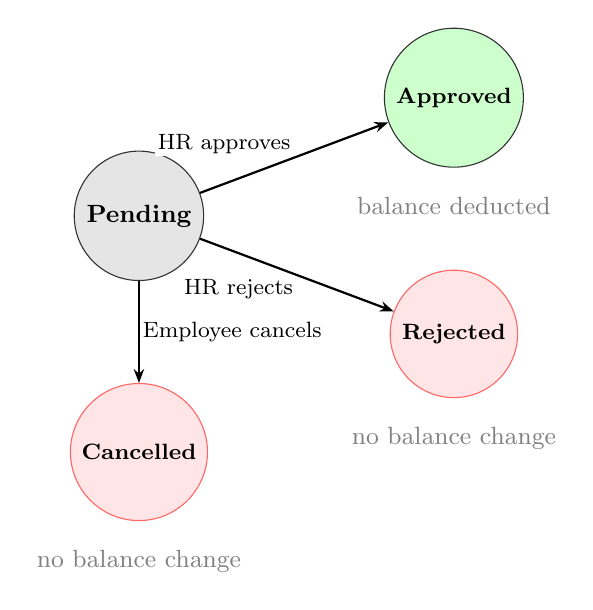
\begin{tikzpicture}[
  state/.style={circle, draw=black!60, fill=white, minimum size=1.2cm, font=\small\bfseries, align=center},
  initstate/.style={circle, draw=black!80, fill=gray!20, minimum size=1.2cm, font=\small\bfseries},
  termstate/.style={circle, draw=black!80, fill=green!20, minimum size=1.1cm, font=\footnotesize\bfseries, align=center},
  dismissstate/.style={circle, draw=red!60, fill=red!10, minimum size=1.1cm, font=\footnotesize\bfseries, align=center},
  arr/.style={-{Stealth[length=5pt]}, thick},
  lbl/.style={font=\footnotesize, fill=white, inner sep=1pt},
]
\node[initstate]  (pending)  at (0,0)     {Pending};
\node[termstate]  (approved) at (4, 1.5)  {Approved};
\node[dismissstate](rejected) at (4,-1.5)  {Rejected};
\node[dismissstate](cancelled) at (0,-3)   {Cancelled};

\draw[arr] (pending)  -- node[lbl, above left]{HR approves} (approved);
\draw[arr] (pending)  -- node[lbl, below left]{HR rejects}  (rejected);
\draw[arr] (pending)  -- node[lbl, right]{Employee cancels} (cancelled);

\node[font=\small, text=gray, below=0.25cm of approved]  {balance deducted};
\node[font=\small, text=gray, below=0.25cm of rejected]  {no balance change};
\node[font=\small, text=gray, below=0.25cm of cancelled] {no balance change};
\end{tikzpicture}
\caption{Leave Request State Machine}
\label{fig:leave_state}
\end{figure}

\subsubsection{Payroll Processing}

\begin{table}[H]
\centering
\caption{Payroll Processing Requirements}
\label{tab:payroll_req}
\begin{tabular}{|p{2.2cm}|p{5cm}|p{5cm}|}
\hline
\textbf{ID} & \textbf{Requirement} & \textbf{Acceptance Criteria} \\
\hline
FR-PAY-01 & HR shall initiate a monthly payroll run & Period (month/year) selected; status: draft, processing, approved \\
\hline
FR-PAY-02 & System shall compute net salary per employee & Gross minus income tax, EOBI, SESSI, leave deductions \\
\hline
FR-PAY-03 & System shall apply FBR 2024--25 tax slabs & Correct tax computed for filer and non-filer employees \\
\hline
FR-PAY-04 & System shall compute EOBI and SESSI contributions & EOBI 0.75\%; SESSI 0.75\% on wages $\leq$ PKR 25,000 \\
\hline
FR-PAY-05 & System shall generate per-employee payslips & All earnings, deductions, and net salary itemised \\
\hline
FR-PAY-06 & Employees shall view and download their payslips & Available on Payslips page and self-service profile \\
\hline
FR-PAY-07 & System shall notify employees when salary is credited & salary\_credited notification dispatched on payroll approval \\
\hline
\end{tabular}
\end{table}

\subsubsection{AI Analytics}

\begin{table}[H]
\centering
\caption{AI Analytics Requirements}
\label{tab:ai_req}
\begin{tabular}{|p{2.2cm}|p{5cm}|p{5cm}|}
\hline
\textbf{ID} & \textbf{Requirement} & \textbf{Acceptance Criteria} \\
\hline
FR-AI-01 & System shall detect payroll fraud indicators & Duplicate bank accounts, salary spikes $>$50\%, ghost employees \\
\hline
FR-AI-02 & System shall detect salary anomalies & Z-score analysis per department and designation \\
\hline
FR-AI-03 & System shall forecast payroll costs & 3-month forecast using trend and seasonal analysis \\
\hline
FR-AI-04 & System shall provide salary recommendations & Market comparison and internal equity analysis \\
\hline
FR-AI-05 & System shall provide an HR chatbot & Intent classification for salary, leave, attendance queries \\
\hline
FR-AI-06 & AI alerts shall be persisted and reviewable & Stored in ai\_alerts table; visible on AI dashboard \\
\hline
\end{tabular}
\end{table}

\subsubsection{Notifications}

\begin{table}[H]
\centering
\caption{Notification Requirements}
\label{tab:notif_req}
\begin{tabular}{|p{2.2cm}|p{5cm}|p{5cm}|}
\hline
\textbf{ID} & \textbf{Requirement} & \textbf{Acceptance Criteria} \\
\hline
FR-NOT-01 & System shall deliver in-app notifications for key events & Leave submitted, approved, rejected, cancelled; salary credited \\
\hline
FR-NOT-02 & Unread count shall display on employee dashboard & Badge updated on every page load \\
\hline
FR-NOT-03 & Employees shall mark notifications as read & Status updated via PATCH endpoint \\
\hline
FR-NOT-04 & Notifications shall persist in reverse chronological order & Latest first; paginated if more than 20 \\
\hline
\end{tabular}
\end{table}

\subsection{Non-Functional Requirements}

\subsubsection{Performance Requirements}
\begin{itemize}
    \item \textbf{NFR-PERF-01:} API responses for standard CRUD operations shall complete within 500\,ms under normal load
    \item \textbf{NFR-PERF-02:} The payroll computation for up to 200 employees shall complete within 10 seconds
    \item \textbf{NFR-PERF-03:} The frontend application shall achieve initial page load within 3 seconds on standard broadband
    \item \textbf{NFR-PERF-04:} AI analysis endpoints shall complete within 5 seconds for datasets of up to 500 employees
\end{itemize}

\subsubsection{Security Requirements}
\begin{itemize}
    \item \textbf{NFR-SEC-01:} All passwords shall be hashed using bcrypt with cost factor 10 minimum
    \item \textbf{NFR-SEC-02:} All API endpoints (except auth) shall require a valid JWT; unauthenticated requests receive HTTP 401
    \item \textbf{NFR-SEC-03:} Role-based access control shall be enforced server-side; frontend role checks are UX convenience only
    \item \textbf{NFR-SEC-04:} Sensitive configuration values shall be stored in \texttt{.env} files and not committed to version control
    \item \textbf{NFR-SEC-05:} All database queries shall use parameterised statements to prevent SQL injection
    \item \textbf{NFR-SEC-06:} Security audit events (login, logout, failed attempts) shall be logged to the \texttt{security\_audit\_log} table
\end{itemize}

\subsubsection{Reliability Requirements}
\begin{itemize}
    \item \textbf{NFR-REL-01:} Database schema changes shall be managed through versioned migration scripts for reproducibility
    \item \textbf{NFR-REL-02:} The backend shall return structured JSON error responses for all foreseeable failure scenarios
    \item \textbf{NFR-REL-03:} AI module failures shall not crash the main payroll operations
\end{itemize}

\subsubsection{Maintainability Requirements}
\begin{itemize}
    \item \textbf{NFR-MAIN-01:} Backend code shall follow a layered architecture: routes, controllers, services, utilities
    \item \textbf{NFR-MAIN-02:} Frontend code shall use TypeScript throughout for compile-time type safety
    \item \textbf{NFR-MAIN-03:} Backend services shall have corresponding Jest unit tests
    \item \textbf{NFR-MAIN-04:} snake\_case to camelCase transformation shall be centralised in \texttt{transformers.js}
\end{itemize}

\subsubsection{Scalability Requirements}
\begin{itemize}
    \item \textbf{NFR-SCAL-01:} The database schema shall support organisations with up to 10,000 employees without structural changes
    \item \textbf{NFR-SCAL-02:} New leave types, salary components, and notification types shall be addable without code changes to existing modules
\end{itemize}

\begin{lessonbox}
Defining non-functional requirements before coding paid dividends. When we initially wrote the payroll computation endpoint without the 10-second performance target, we processed employees sequentially. Adding the requirement forced us to analyse the query patterns and batch the computation, which reduced processing time for 200 employees from 45 seconds to 3.8 seconds.
\end{lessonbox}

\section{System Architecture Design}

Figure~\ref{fig:architecture} illustrates the high-level system architecture of PayrollX, showing the two primary user roles and their interactions with system modules, backed by the centralised PostgreSQL database.

\begin{figure}[H]
\centering
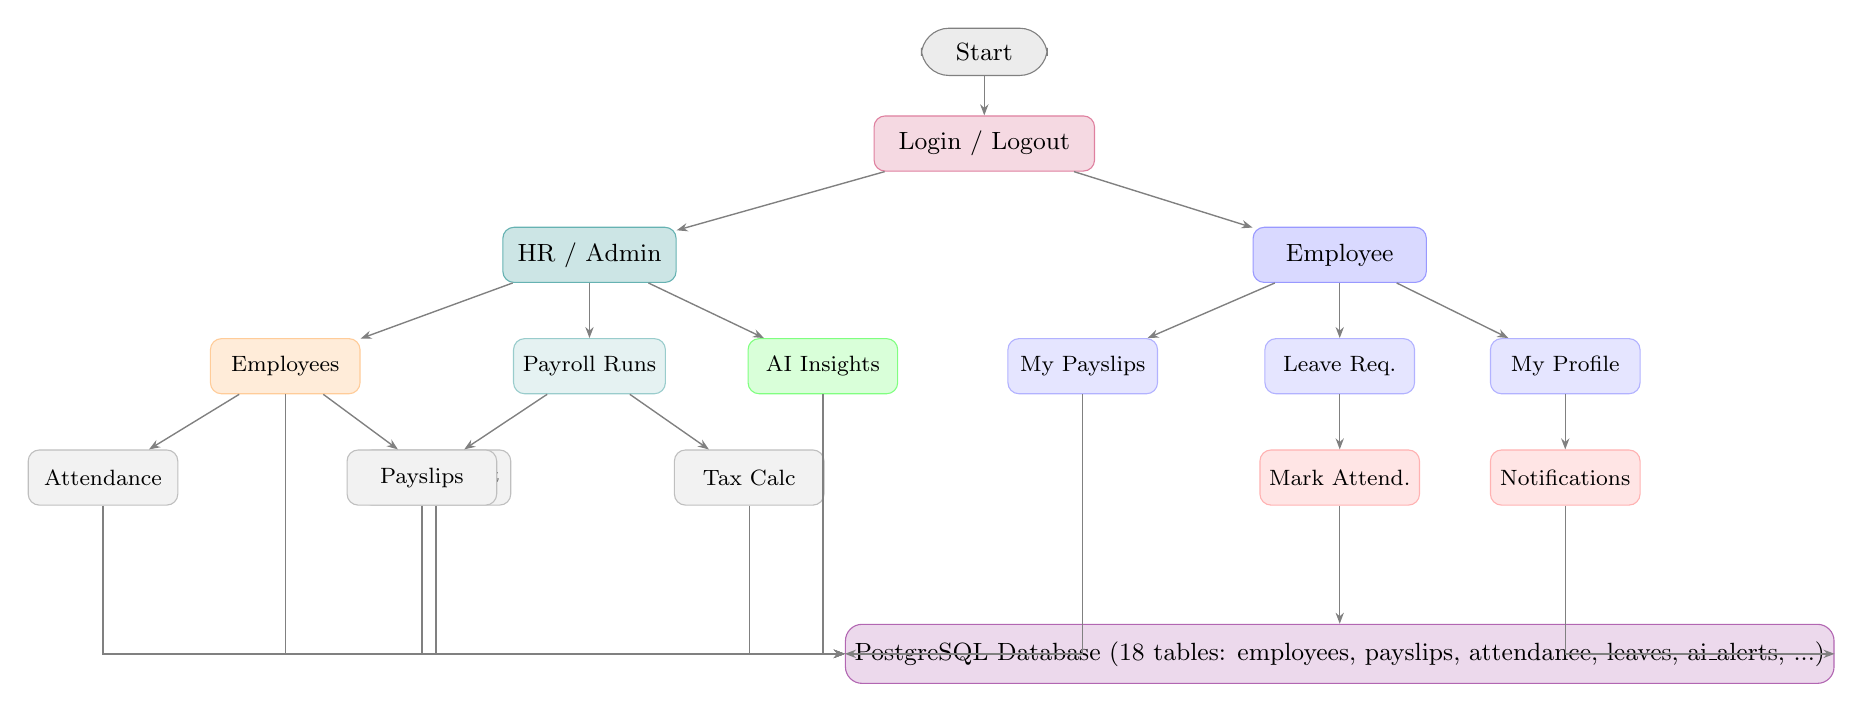
\begin{tikzpicture}[
  node distance=0.55cm and 0.4cm,
  every node/.style={font=\small},
  box/.style={rectangle, rounded corners=4pt, draw=black!50, fill=white, text centered, minimum height=0.7cm, minimum width=2.2cm, line width=0.4pt},
  startbox/.style={rectangle, rounded corners=10pt, draw=black!50, fill=gray!15, text centered, minimum height=0.6cm, minimum width=1.6cm, line width=0.4pt},
  hrbox/.style={box, fill=teal!20, draw=teal!60},
  empbox/.style={box, fill=blue!15, draw=blue!40},
  subhrbox/.style={box, fill=teal!10, draw=teal!40, minimum width=1.9cm, font=\footnotesize},
  subempbox/.style={box, fill=blue!10, draw=blue!30, minimum width=1.9cm, font=\footnotesize},
  leafbox/.style={box, fill=gray!10, draw=gray!50, minimum width=1.9cm, font=\footnotesize},
  dbbox/.style={rectangle, rounded corners=6pt, draw=violet!60, fill=violet!15, text centered, minimum height=0.75cm, line width=0.4pt},
  authbox/.style={box, fill=purple!15, draw=purple!50, minimum width=2.8cm},
  amberbox/.style={box, fill=orange!15, draw=orange!40, minimum width=1.9cm, font=\footnotesize},
  coralbox/.style={box, fill=red!10, draw=red!30, minimum width=1.9cm, font=\footnotesize},
  aibox/.style={box, fill=green!15, draw=green!50, minimum width=1.9cm, font=\footnotesize},
  arr/.style={-{Stealth[length=4pt]}, draw=black!50, line width=0.5pt},
]

%% Row 0: Start
\node[startbox] (start) {Start};

%% Row 1: Login
\node[authbox, below=0.5cm of start] (login) {Login / Logout};

%% Row 2: HR and Employee
\node[hrbox,  below left=0.7cm and 2.5cm of login] (hr)  {HR / Admin};
\node[empbox, below right=0.7cm and 2.0cm of login] (emp) {Employee};

%% HR sub-nodes
\node[amberbox, below left=0.7cm and 1.8cm of hr]   (empmod)   {Employees};
\node[subhrbox, below=0.7cm of hr]                   (paymod) {Payroll Runs};
\node[aibox, below right=0.7cm and 0.9cm of hr]     (aimod)   {AI Insights};

%% HR leaf nodes
\node[leafbox, below left=0.7cm and 0.4cm of empmod]  (atthr)    {Attendance};
\node[leafbox, below right=0.7cm and 0.0cm of empmod] (leavemod) {Leave Mgmt};
\node[leafbox, below left=0.7cm and 0.2cm of paymod]  (paysliphr){Payslips};
\node[leafbox, below right=0.7cm and 0.1cm of paymod] (taxmod)   {Tax Calc};

%% Employee sub-nodes
\node[subempbox, below left=0.7cm and 1.2cm of emp]   (mypay) {My Payslips};
\node[subempbox, below=0.7cm of emp]                   (leavereq){Leave Req.};
\node[subempbox, below right=0.7cm and 0.8cm of emp]  (profile) {My Profile};

%% Employee leaf nodes
\node[coralbox, below=0.7cm of leavereq]  (attemp) {Mark Attend.};
\node[coralbox, below=0.7cm of profile]   (notif)  {Notifications};

%% Database
\node[dbbox, below=1.5cm of attemp, minimum width=11cm] (db) {PostgreSQL Database (18 tables: employees, payslips, attendance, leaves, ai\_alerts, ...)};

%% Arrows
\draw[arr] (start)    -- (login);
\draw[arr] (login)    -- (hr);
\draw[arr] (login)    -- (emp);
\draw[arr] (hr)       -- (empmod);
\draw[arr] (hr)       -- (paymod);
\draw[arr] (hr)       -- (aimod);
\draw[arr] (empmod)   -- (atthr);
\draw[arr] (empmod)   -- (leavemod);
\draw[arr] (paymod)   -- (paysliphr);
\draw[arr] (paymod)   -- (taxmod);
\draw[arr] (emp)      -- (mypay);
\draw[arr] (emp)      -- (leavereq);
\draw[arr] (emp)      -- (profile);
\draw[arr] (leavereq) -- (attemp);
\draw[arr] (profile)  -- (notif);
\draw[arr] (empmod)     |- (db);
\draw[arr] (atthr)      |- (db);
\draw[arr] (leavemod)   |- (db);
\draw[arr] (paysliphr)  |- (db);
\draw[arr] (taxmod)     |- (db);
\draw[arr] (aimod)      |- (db);
\draw[arr] (mypay)      |- (db);
\draw[arr] (attemp)     -- (db);
\draw[arr] (notif)      |- (db);

\end{tikzpicture}
\caption{PayrollX System Architecture Overview}
\label{fig:architecture}
\end{figure}

\subsection{Backend Architecture}

The backend is structured using a layered architecture that enforces strict separation of concerns across four layers:

\begin{itemize}
    \item \textbf{Routes Layer} (\texttt{server/src/routes/}): Defines HTTP endpoint URLs, applies validation middleware, and delegates to controllers. There are 10 route groups: auth, employees, attendance, leaves, departments, payroll, ai, notifications, settings, dashboard.
    \item \textbf{Controllers Layer} (\texttt{server/src/controllers/}): Handles request parsing, calls service methods, and formats API responses using the \texttt{apiResponse} utility. Controllers contain no business logic.
    \item \textbf{Services Layer} (\texttt{server/src/services/}): Encapsulates all business logic. Key services are \texttt{employee.service.js}, \texttt{attendance.service.js}, \texttt{leave.service.js}, \texttt{payroll.service.js}, \texttt{notification.service.js}, and five AI services under \texttt{services/ai/}.
    \item \textbf{Utilities Layer} (\texttt{server/src/utils/}): Contains the FBR tax calculator (\texttt{taxCalculator.js}), data transformers (\texttt{transformers.js}), custom error classes (\texttt{errors.js}), and the \texttt{apiResponse} formatter.
\end{itemize}

Authentication and authorisation are enforced at the middleware layer (\texttt{server/src/middleware/}) before requests reach controllers.

\subsection{Frontend Architecture}

The React frontend follows a layered component architecture:

\begin{itemize}
    \item \textbf{Pages} (\texttt{src/pages/}): 14 page components including \texttt{HrDashboard.tsx}, \texttt{EmployeeDashboard.tsx}, \texttt{Employees.tsx}, \texttt{Attendance.tsx}, \texttt{Leaves.tsx}, \texttt{Payroll.tsx}, \texttt{Payslips.tsx}, \texttt{AIInsights.tsx}, \texttt{MyProfile.tsx}, \texttt{Settings.tsx}.
    \item \textbf{Hooks} (\texttt{src/hooks/}): Custom TanStack Query hooks (\texttt{useAuth.ts}, \texttt{useEmployees.ts}, \texttt{useAttendance.ts}, \texttt{useLeaves.ts}, \texttt{usePayroll.ts}, \texttt{useAI.ts}, \texttt{useNotifications.ts}) encapsulate all API calls and server state caching.
    \item \textbf{Components} (\texttt{src/components/}): shadcn/ui component library plus custom layout wrappers and reusable UI building blocks.
    \item \textbf{Store} (\texttt{src/store/}): Redux Toolkit slices for client-side state (session context, UI preferences).
    \item \textbf{Library} (\texttt{src/lib/}): The centralised Axios API client (\texttt{api.ts}) with JWT interceptor and auto-refresh logic.
\end{itemize}

\section{Database Design}

The PostgreSQL database is managed through 18 versioned migration files. Table~\ref{tab:db_tables} summarises the core entities.

\begin{table}[H]
\centering
\caption{Database Tables and Their Purpose}
\label{tab:db_tables}
\begin{tabular}{|l|p{9cm}|}
\hline
\textbf{Table} & \textbf{Purpose} \\
\hline
\texttt{users}             & Authentication credentials and role (admin, hr, employee) \\
\hline
\texttt{departments}       & Company departments \\
\hline
\texttt{employees}         & Full employee records linked to users and departments \\
\hline
\texttt{salary\_structures} & Salary component breakdowns per employee \\
\hline
\texttt{attendance}        & Daily attendance events with timestamp and status \\
\hline
\texttt{leave\_types}      & Configurable leave categories (annual, sick, casual, etc.) \\
\hline
\texttt{leave\_requests}   & Individual leave applications with status lifecycle \\
\hline
\texttt{leave\_allocations} & Per-employee leave balances per leave type per year \\
\hline
\texttt{payroll\_runs}     & Monthly payroll processing batches with status \\
\hline
\texttt{payslips}          & Computed payslips with all earnings and deductions \\
\hline
\texttt{ai\_alerts}        & Fraud and anomaly alerts generated by AI modules \\
\hline
\texttt{chatbot\_sessions} / \texttt{chatbot\_messages} & HR chatbot conversation logs \\
\hline
\texttt{public\_holidays}  & Pakistani public holiday calendar \\
\hline
\texttt{refresh\_tokens}   & JWT refresh token storage for rotation \\
\hline
\texttt{security\_audit\_log} & Security event log (login, logout, failed attempts) \\
\hline
\texttt{notifications}     & In-app notification records per employee \\
\hline
\texttt{settings}          & System configuration key-value pairs \\
\hline
\end{tabular}
\end{table}

\subsection{Key Relationships}

\begin{itemize}
    \item Each \texttt{employee} belongs to one \texttt{department} and is linked to one \texttt{user} account.
    \item Each \texttt{attendance} record belongs to one \texttt{employee}.
    \item Each \texttt{leave\_request} belongs to one \texttt{employee} and references one \texttt{leave\_type}.
    \item Each \texttt{leave\_allocation} belongs to one \texttt{employee} and one \texttt{leave\_type}.
    \item Each \texttt{payslip} belongs to one \texttt{employee} and one \texttt{payroll\_run}.
    \item Each \texttt{notification} belongs to one \texttt{employee}.
    \item Each \texttt{ai\_alert} references one \texttt{employee} and specifies an alert type.
\end{itemize}

\begin{figure}[H]
\centering
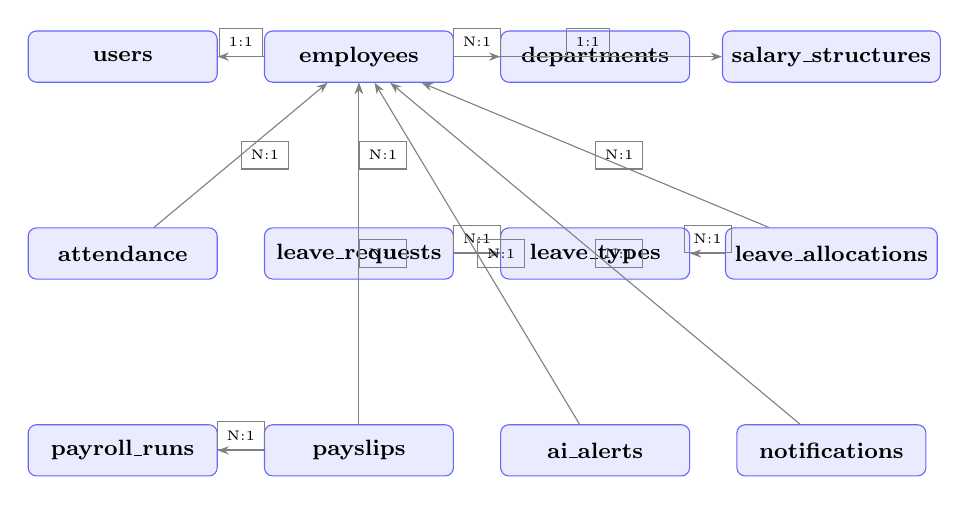
\begin{tikzpicture}[
  ent/.style={rectangle, draw=blue!60, fill=blue!8, rounded corners=3pt, minimum width=2.4cm, minimum height=0.65cm, font=\footnotesize\bfseries, align=center},
  rel/.style={draw=black!50, font=\tiny},
  arr/.style={-{Stealth[length=4pt]}, draw=black!50},
  node distance=1.6cm and 2.2cm,
]
%% Core entities
\node[ent] (users)      at (0,0)        {users};
\node[ent] (employees)  at (3,0)        {employees};
\node[ent] (depts)      at (6,0)        {departments};
\node[ent] (salaries)   at (9,0)        {salary\_structures};

\node[ent] (attendance) at (0,-2.5)     {attendance};
\node[ent] (lreq)       at (3,-2.5)     {leave\_requests};
\node[ent] (ltypes)     at (6,-2.5)     {leave\_types};
\node[ent] (lalloc)     at (9,-2.5)     {leave\_allocations};

\node[ent] (pruns)      at (0,-5)       {payroll\_runs};
\node[ent] (payslips)   at (3,-5)       {payslips};
\node[ent] (aialerts)   at (6,-5)       {ai\_alerts};
\node[ent] (notifs)     at (9,-5)       {notifications};

%% Row 1 relations
\draw[arr] (employees) -- node[above,rel]{1:1} (users);
\draw[arr] (employees) -- node[above,rel]{N:1} (depts);
\draw[arr] (employees) -- node[above,rel]{1:1} (salaries);

%% Row 2 relations
\draw[arr] (attendance) -- node[right,rel]{N:1} (employees);
\draw[arr] (lreq)       -- node[right,rel]{N:1} (employees);
\draw[arr] (lreq)       -- node[above,rel]{N:1} (ltypes);
\draw[arr] (lalloc)     -- node[right,rel]{N:1} (employees);
\draw[arr] (lalloc)     -- node[above,rel]{N:1} (ltypes);

%% Row 3 relations
\draw[arr] (payslips)   -- node[above,rel]{N:1} (pruns);
\draw[arr] (payslips)   -- node[right,rel]{N:1} (employees);
\draw[arr] (aialerts)   -- node[right,rel]{N:1} (employees);
\draw[arr] (notifs)     -- node[right,rel]{N:1} (employees);
\end{tikzpicture}
\caption{Simplified Entity-Relationship Diagram (Key Tables)}
\label{fig:er_diagram}
\end{figure}

\section{API Design}

PayrollX implements a RESTful API with consistent conventions. Table~\ref{tab:api_groups} summarises the API endpoint groups.

\begin{table}[H]
\centering
\caption{API Endpoint Groups}
\label{tab:api_groups}
\begin{tabular}{|l|l|p{7cm}|}
\hline
\textbf{Group} & \textbf{Base Path} & \textbf{Key Endpoints} \\
\hline
Auth          & \texttt{/api/v1/auth}        & POST /login, POST /logout, POST /refresh, GET /me \\
\hline
Employees     & \texttt{/api/v1/employees}   & CRUD + GET /stats \\
\hline
Attendance    & \texttt{/api/v1/attendance}  & POST /check-in, POST /check-out, POST /mark, GET /daily-stats \\
\hline
Leaves        & \texttt{/api/v1/leaves}      & CRUD + POST /:id/approve, POST /:id/reject, GET /balance/:id \\
\hline
Departments   & \texttt{/api/v1/departments} & CRUD \\
\hline
Payroll       & \texttt{/api/v1/payroll}     & GET /runs, POST /runs, POST /runs/:id/process, GET /payslips, POST /calculate-tax \\
\hline
AI            & \texttt{/api/v1/ai}          & GET /dashboard, GET /alerts, POST /fraud-detection/run, POST /salary-anomaly/detect, GET /forecast, POST /chatbot \\
\hline
Notifications & \texttt{/api/v1/notifications} & GET /, PATCH /:id/read, POST /read-all \\
\hline
Settings      & \texttt{/api/v1/settings}    & GET /, PUT /, GET /holidays, POST /holidays \\
\hline
Dashboard     & \texttt{/api/v1/dashboard}   & GET /hr, GET /employee \\
\hline
\end{tabular}
\end{table}

All API responses follow the standard format illustrated in Figure~\ref{fig:api_response}.

\begin{figure}[H]
\centering
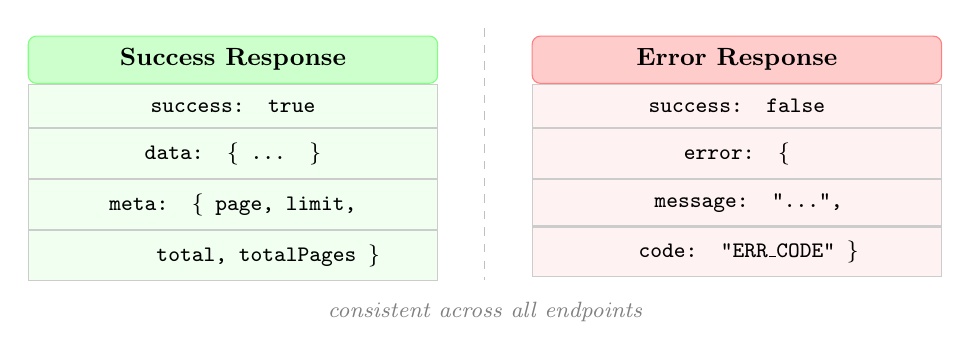
\begin{tikzpicture}[
  hdr/.style={rectangle, draw=black!40, fill=gray!15, rounded corners=3pt, minimum width=5.2cm, minimum height=0.6cm, font=\small\bfseries, align=center},
  row/.style={rectangle, draw=black!20, fill=white, minimum width=5.2cm, minimum height=0.55cm, font=\ttfamily\footnotesize, align=left, inner sep=5pt},
  greenrow/.style={row, fill=green!6},
  redrow/.style={row, fill=red!5},
  node distance=0cm,
]
\node[hdr, fill=green!20, draw=green!50] (sh) at (-3.2, 0) {Success Response};
\node[greenrow, below=0cm of sh] (s1) {\texttt{success: true}};
\node[greenrow, below=0cm of s1] (s2) {\texttt{data: \{ ... \}}};
\node[greenrow, below=0cm of s2] (s3) {\texttt{meta: \{ page, limit,}};
\node[greenrow, below=0cm of s3] (s4) {\texttt{\quad\quad\quad total, totalPages \}}};

\node[hdr, fill=red!20, draw=red!50] (eh) at (3.2, 0) {Error Response};
\node[redrow, below=0cm of eh] (e1) {\texttt{success: false}};
\node[redrow, below=0cm of e1] (e2) {\texttt{error: \{}};
\node[redrow, below=0cm of e2] (e3) {\texttt{\quad message: "...",}};
\node[redrow, below=0cm of e3] (e4) {\texttt{\quad code: "ERR\_CODE" \}}};

\draw[dashed, gray!50] (0, 0.4) -- (0,-2.8);
\node[font=\footnotesize\itshape, text=gray] at (0,-3.2) {consistent across all endpoints};
\end{tikzpicture}
\caption{Standard API Response Format --- Success and Error Envelopes}
\label{fig:api_response}
\end{figure}

% ============================================================================
% CHAPTER 4: IMPLEMENTATION
% ============================================================================
\chapter{Implementation}
\label{chap:implementation}

This chapter details the implementation of all components of PayrollX, from the backend authentication layer to the AI modules and the React frontend.

\section{Development Stages}

\subsection{Stage 1: Project Scaffolding and Authentication}

The first stage established the backend and frontend project structure. The Express.js backend was initialised with a directory layout separating routes, controllers, services, middleware, and utilities. PostgreSQL was connected via the \texttt{pg} (node-postgres) library using a connection pool for performance.

JWT-based authentication was the first functional feature implemented. The login endpoint validates credentials, compares the password using bcrypt, and returns both an access token (15-minute expiry) and a rotating refresh token (7-day expiry). The authentication middleware validates the access token on every protected route.

Figure~\ref{fig:auth_usecase} shows the authentication use cases for each actor. Figure~\ref{fig:auth_flow} shows the complete JWT authentication sequence including token refresh.

\begin{figure}[H]
\centering
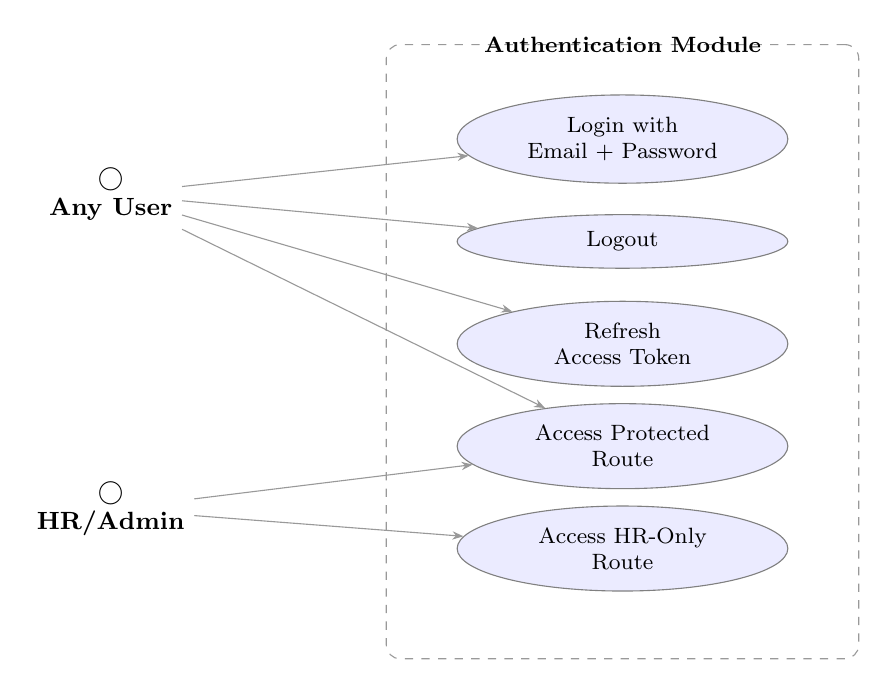
\begin{tikzpicture}[
  uc/.style={ellipse, draw=black!50, fill=blue!8, font=\footnotesize, align=center, minimum width=4.2cm, minimum height=0.65cm},
  sysbox/.style={rectangle, draw=black!40, minimum width=6cm, minimum height=7.8cm, dashed, rounded corners=5pt},
  arr/.style={draw=black!40, -{Stealth[length=4pt]}},
  lbl/.style={font=\tiny, text=gray},
]
\node[sysbox] at (5.2,-3.5) {};
\node[font=\footnotesize\bfseries] at (5.2,0.4) {Authentication Module};

\node[font=\small\bfseries, align=center] (ua) at (-1.3,-1.5) {$\bigcirc$\\\small Any User};
\node[font=\small\bfseries, align=center] (ha) at (-1.3,-5.5) {$\bigcirc$\\\small HR/Admin};

\node[uc] (login)   at (5.2,-0.8) {Login with\\Email + Password};
\node[uc] (logout)  at (5.2,-2.1) {Logout};
\node[uc] (refresh) at (5.2,-3.4) {Refresh\\Access Token};
\node[uc] (protect) at (5.2,-4.7) {Access Protected\\Route};
\node[uc] (hronly)  at (5.2,-6.0) {Access HR-Only\\Route};

\draw[arr] (ua) -- (login);
\draw[arr] (ua) -- (logout);
\draw[arr] (ua) -- (refresh);
\draw[arr] (ua) -- (protect);
\draw[arr] (ha) -- (hronly);
\draw[arr] (ha) -- (protect);
\end{tikzpicture}
\caption{Authentication Module Use Case Diagram}
\label{fig:auth_usecase}
\end{figure}

\begin{figure}[H]
\centering
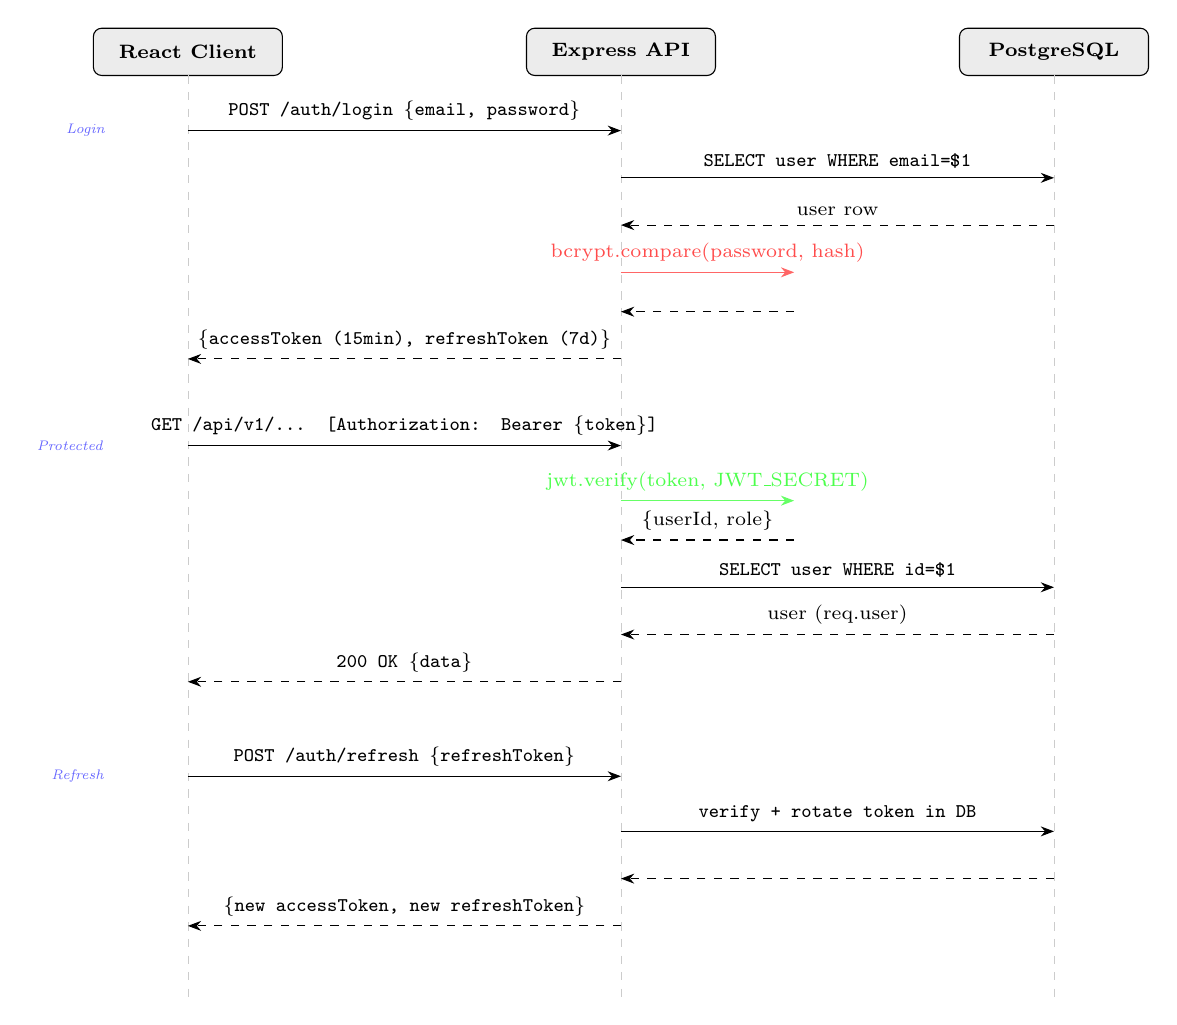
\begin{tikzpicture}[
  actor/.style={draw, rounded corners=3pt, fill=gray!15, minimum width=2.4cm, minimum height=0.6cm, align=center, font=\scriptsize\bfseries},
  msg/.style={->, >=Stealth, font=\scriptsize},
  retmsg/.style={->, >=Stealth, dashed, font=\scriptsize},
  lifeline/.style={draw=gray!40, dashed, very thin},
]

% Actors
\node[actor] (client) at (0,0)    {React Client};
\node[actor] (api)    at (5.5,0)  {Express API};
\node[actor] (db)     at (11,0)   {PostgreSQL};

% Lifelines
\draw[lifeline] (0,-0.3)   -- (0,-12);
\draw[lifeline] (5.5,-0.3) -- (5.5,-12);
\draw[lifeline] (11,-0.3)  -- (11,-12);

% Login flow
\draw[msg]    (0,-1.0) -- node[above]{\texttt{POST /auth/login \{email, password\}}} (5.5,-1.0);
\draw[msg]    (5.5,-1.6) -- node[above]{\texttt{SELECT user WHERE email=\$1}} (11,-1.6);
\draw[retmsg] (11,-2.2) -- node[above]{user row} (5.5,-2.2);
\draw[msg, draw=red!60] (5.5,-2.8) -- node[above, text=red!70]{\scriptsize bcrypt.compare(password, hash)} ++(2.2,0);
\draw[retmsg] (7.7,-3.3) -- (5.5,-3.3);
\draw[retmsg] (5.5,-3.9) -- node[above]{\texttt{\{accessToken (15min), refreshToken (7d)\}}} (0,-3.9);

% Protected route
\draw[msg]    (0,-5.0) -- node[above]{\texttt{GET /api/v1/... [Authorization: Bearer \{token\}]}} (5.5,-5.0);
\draw[msg, draw=green!60] (5.5,-5.7) -- node[above, text=green!70]{\scriptsize jwt.verify(token, JWT\_SECRET)} ++(2.2,0);
\draw[retmsg] (7.7,-6.2) -- node[above]{\scriptsize \{userId, role\}} (5.5,-6.2);
\draw[msg]    (5.5,-6.8) -- node[above]{\texttt{SELECT user WHERE id=\$1}} (11,-6.8);
\draw[retmsg] (11,-7.4) -- node[above]{user (req.user)} (5.5,-7.4);
\draw[retmsg] (5.5,-8.0) -- node[above]{\texttt{200 OK \{data\}}} (0,-8.0);

% Token refresh
\draw[msg]    (0,-9.2) -- node[above]{\texttt{POST /auth/refresh \{refreshToken\}}} (5.5,-9.2);
\draw[msg]    (5.5,-9.9) -- node[above]{\texttt{verify + rotate token in DB}} (11,-9.9);
\draw[retmsg] (11,-10.5) -- (5.5,-10.5);
\draw[retmsg] (5.5,-11.1) -- node[above]{\texttt{\{new accessToken, new refreshToken\}}} (0,-11.1);

\node[font=\tiny\itshape, text=blue!60] at (-1.3,-1.0) {Login};
\node[font=\tiny\itshape, text=blue!60] at (-1.5,-5.0) {Protected};
\node[font=\tiny\itshape, text=blue!60] at (-1.4,-9.2) {Refresh};

\end{tikzpicture}
\caption{JWT Authentication Sequence Diagram}
\label{fig:auth_flow}
\end{figure}

\subsection{Stage 2: Employee and Department Management}

With authentication in place, employee management was implemented. The \texttt{employee.service.js} provides functions to create, list, retrieve, update, and soft-delete employee records. Salary structures are stored in a separate \texttt{salary\_structures} table, normalising the relationship between employees and their compensation components.

The \texttt{transformers.js} utility performs all snake\_case to camelCase conversion, ensuring the backend database naming convention does not leak into the frontend API contract.

\begin{failbox}
Our initial employee creation endpoint accepted the salary structure fields as part of the same request body and inserted them in a single SQL statement. This worked until we needed to update salary structures independently. We refactored to a separate \texttt{salary\_structures} table with its own CRUD, which required a data migration and a frontend change. Designing the database schema carefully before writing code would have avoided this refactor.
\end{failbox}

\subsection{Stage 3: Attendance and Leave Management}

Attendance and leave modules were developed together because of their interdependency in payroll computation. \texttt{attendance.service.js} handles check-in and check-out recording with duplicate prevention: an employee cannot check in twice on the same day without first checking out.

Leave management required the most complex state machine: a leave request transitions through \texttt{pending} $\to$ \texttt{approved}/\texttt{rejected} (by HR) or \texttt{cancelled} (by employee). Approved requests trigger an automatic balance deduction in \texttt{leave\_allocations}. Notification events for each state transition are dispatched by calling \texttt{notification.service.js} after the state change is persisted.

\subsection{Stage 4: Payroll Processing and FBR Tax Compliance}

The payroll module is the most business-critical component. When HR initiates a payroll run for a month, \texttt{payroll.service.js} iterates over all active employees and computes net salary using the following algorithm:

Figure~\ref{fig:payroll_usecase} shows the payroll module use cases; Figure~\ref{fig:payroll_flow} illustrates the complete computation flow for a single payroll run.

\begin{figure}[H]
\centering
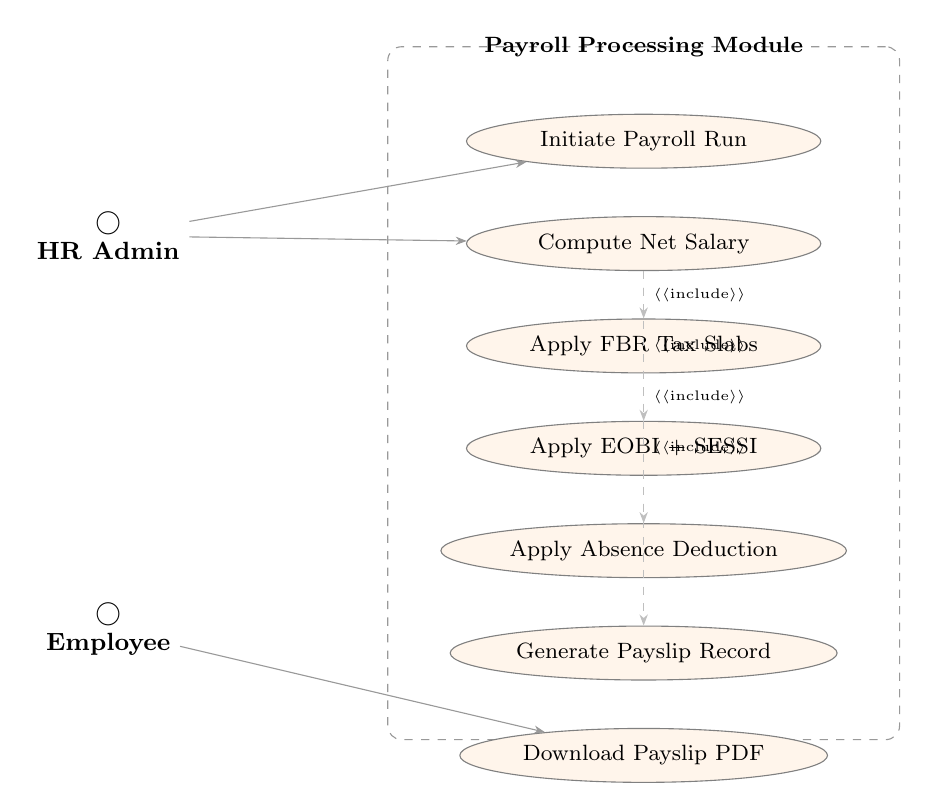
\begin{tikzpicture}[
  uc/.style={ellipse, draw=black!50, fill=orange!8, font=\footnotesize, align=center, minimum width=4.5cm, minimum height=0.65cm},
  sysbox/.style={rectangle, draw=black!40, minimum width=6.5cm, minimum height=8.8cm, dashed, rounded corners=5pt},
  arr/.style={draw=black!40, -{Stealth[length=4pt]}},
  incl/.style={draw=gray!50, dashed, -{Stealth[length=4pt]}, font=\tiny},
]
\node[sysbox] at (5.5,-4) {};
\node[font=\footnotesize\bfseries] at (5.5,0.4) {Payroll Processing Module};

\node[font=\small\bfseries, align=center] (hr) at (-1.3,-2)  {$\bigcirc$\\\small HR Admin};
\node[font=\small\bfseries, align=center] (emp) at (-1.3,-7) {$\bigcirc$\\\small Employee};

\node[uc] (init)     at (5.5,-0.8) {Initiate Payroll Run};
\node[uc] (compute)  at (5.5,-2.1) {Compute Net Salary};
\node[uc] (tax)      at (5.5,-3.4) {Apply FBR Tax Slabs};
\node[uc] (contrib)  at (5.5,-4.7) {Apply EOBI + SESSI};
\node[uc] (absence)  at (5.5,-6.0) {Apply Absence Deduction};
\node[uc] (payslip)  at (5.5,-7.3) {Generate Payslip Record};
\node[uc] (download) at (5.5,-8.6) {Download Payslip PDF};

\draw[arr] (hr)  -- (init);
\draw[arr] (hr)  -- (compute);
\draw[arr] (emp) -- (download);
\draw[incl] (compute) -- node[right]{$\langle\langle$include$\rangle\rangle$} (tax);
\draw[incl] (compute) -- node[right]{$\langle\langle$include$\rangle\rangle$} (contrib);
\draw[incl] (compute) -- node[right]{$\langle\langle$include$\rangle\rangle$} (absence);
\draw[incl] (compute) -- node[right]{$\langle\langle$include$\rangle\rangle$} (payslip);
\end{tikzpicture}
\caption{Payroll Processing Module Use Case Diagram}
\label{fig:payroll_usecase}
\end{figure}

\begin{figure}[H]
\centering
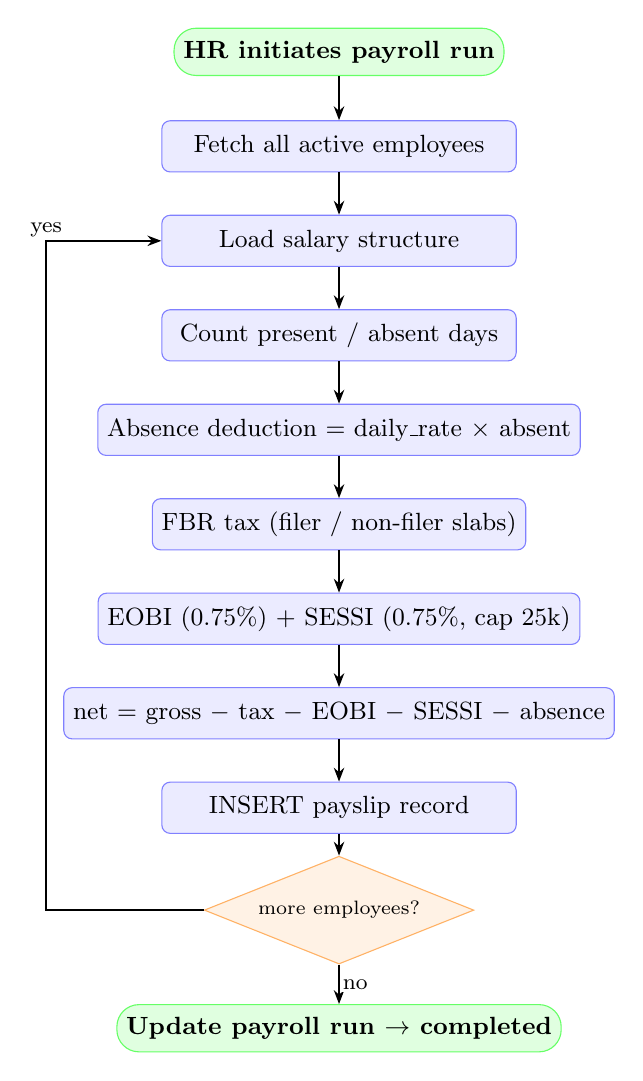
\begin{tikzpicture}[
  proc/.style={rectangle, draw=blue!50, fill=blue!8, rounded corners=3pt, minimum width=4.5cm, minimum height=0.65cm, font=\small, align=center},
  dec/.style={diamond, draw=orange!60, fill=orange!10, minimum width=3cm, minimum height=0.9cm, font=\scriptsize, align=center, aspect=2.5},
  term/.style={rectangle, draw=green!60, fill=green!12, rounded corners=8pt, minimum width=3cm, minimum height=0.6cm, font=\small\bfseries},
  arr/.style={-{Stealth[length=5pt]}, thick},
  lbl/.style={font=\footnotesize, fill=white, inner sep=1pt},
  node distance=0.6cm,
]
\node[term]  (start)  at (0,0)     {HR initiates payroll run};
\node[proc]  (fetch)  at (0,-1.2)  {Fetch all active employees};
\node[proc]  (sal)    at (0,-2.4)  {Load salary structure};
\node[proc]  (att)    at (0,-3.6)  {Count present / absent days};
\node[proc]  (abs)    at (0,-4.8)  {Absence deduction = daily\_rate $\times$ absent};
\node[proc]  (tax)    at (0,-6.0)  {FBR tax (filer / non-filer slabs)};
\node[proc]  (stat)   at (0,-7.2)  {EOBI (0.75\%) + SESSI (0.75\%, cap 25k)};
\node[proc]  (net)    at (0,-8.4)  {net = gross $-$ tax $-$ EOBI $-$ SESSI $-$ absence};
\node[proc]  (slip)   at (0,-9.6)  {INSERT payslip record};
\node[dec]   (more)   at (0,-10.9) {more employees?};
\node[term]  (done)   at (0,-12.4) {Update payroll run $\to$ completed};

\draw[arr] (start) -- (fetch);
\draw[arr] (fetch) -- (sal);
\draw[arr] (sal)   -- (att);
\draw[arr] (att)   -- (abs);
\draw[arr] (abs)   -- (tax);
\draw[arr] (tax)   -- (stat);
\draw[arr] (stat)  -- (net);
\draw[arr] (net)   -- (slip);
\draw[arr] (slip)  -- (more);
\draw[arr] (more)  -- node[lbl,right]{no}  (done);
\draw[arr] (more.west) -- ++(-2,0) |- node[lbl,above]{yes} (sal.west);
\end{tikzpicture}
\caption{Payroll Computation Flowchart (per payroll run)}
\label{fig:payroll_flow}
\end{figure}

The FBR tax calculator implements the 2024--25 tax slabs for both filers and non-filers. Table~\ref{tab:fbr_slabs} lists the slab rates; Figure~\ref{fig:tax_flowchart} shows the computation logic.

\begin{table}[H]
\centering
\caption{FBR Income Tax Slabs 2024--25 (Salaried Filers)}
\label{tab:fbr_slabs}
\begin{tabular}{|c|l|c|c|}
\hline
\textbf{Slab} & \textbf{Annual Income (PKR)} & \textbf{Rate} & \textbf{Base Tax (PKR)} \\
\hline
1 & Up to 600,000              & 0\%    & 0 \\
\hline
2 & 600,001 -- 1,200,000       & 2.5\%  & 0 \\
\hline
3 & 1,200,001 -- 2,200,000     & 12.5\% & 15,000 \\
\hline
4 & 2,200,001 -- 3,200,000     & 22.5\% & 140,000 \\
\hline
5 & 3,200,001 -- 4,100,000     & 27.5\% & 365,000 \\
\hline
6 & Above 4,100,000            & 35\%   & 612,500 \\
\hline
\multicolumn{4}{|l|}{\footnotesize Non-filers pay $\approx$10\% surcharge on top of filer tax} \\
\hline
\end{tabular}
\end{table}

\begin{figure}[H]
\centering
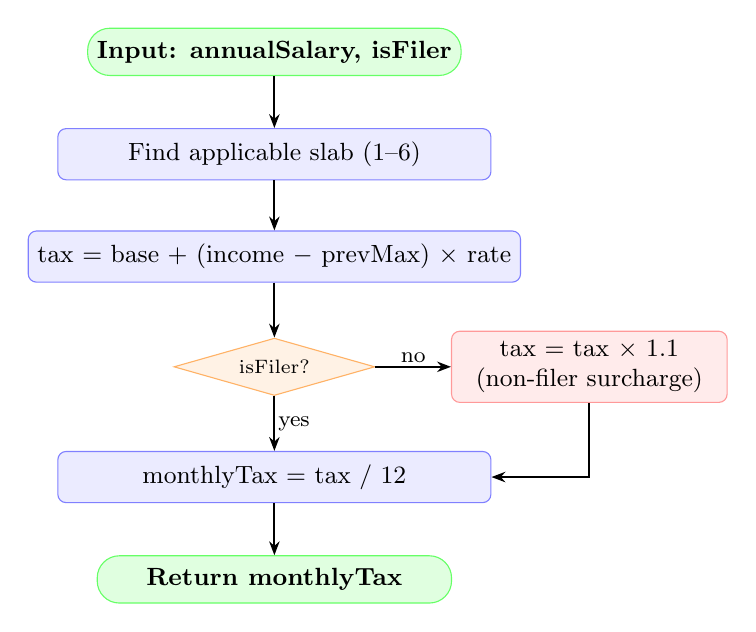
\begin{tikzpicture}[
  proc/.style={rectangle, draw=blue!50, fill=blue!8, rounded corners=3pt, minimum width=5.5cm, minimum height=0.65cm, font=\small, align=center},
  dec/.style={diamond, draw=orange!60, fill=orange!10, font=\scriptsize, align=center, aspect=3.5},
  term/.style={rectangle, draw=green!60, fill=green!12, rounded corners=8pt, minimum width=4.5cm, minimum height=0.6cm, font=\small\bfseries, align=center},
  surbox/.style={rectangle, draw=red!40, fill=red!8, rounded corners=3pt, minimum width=3.5cm, minimum height=0.65cm, font=\small, align=center},
  arr/.style={-{Stealth[length=5pt]}, thick},
  lbl/.style={font=\footnotesize, fill=white, inner sep=1pt},
  node distance=0.7cm,
]
\node[term]  (start)    at (0,0)    {Input: annualSalary, isFiler};
\node[proc]  (slab)     at (0,-1.3) {Find applicable slab (1--6)};
\node[proc]  (calc)     at (0,-2.6) {tax = base + (income $-$ prevMax) $\times$ rate};
\node[dec]   (filer)    at (0,-4.0) {isFiler?};
\node[surbox](surcharge) at (4,-4.0) {tax = tax $\times$ 1.1\\(non-filer surcharge)};
\node[proc]  (monthly)  at (0,-5.4) {monthlyTax = tax / 12};
\node[term]  (out)      at (0,-6.7) {Return monthlyTax};

\draw[arr] (start) -- (slab);
\draw[arr] (slab)  -- (calc);
\draw[arr] (calc)  -- (filer);
\draw[arr] (filer) -- node[lbl,above]{no} (surcharge);
\draw[arr] (filer) -- node[lbl,right]{yes} (monthly);
\draw[arr] (surcharge) |- (monthly);
\draw[arr] (monthly) -- (out);
\end{tikzpicture}
\caption{FBR Tax Computation Flowchart}
\label{fig:tax_flowchart}
\end{figure}

\subsection{Stage 5: AI Analytics Modules}

Five AI service modules live in \texttt{server/src/services/ai/}. Rule-based and statistical algorithms were chosen over ML for three reasons: interpretability (HR decisions must be auditable), limited data volume at SME scale, and zero model-serving infrastructure.

\subsubsection{Fraud Detection --- 10 Algorithms}

Table~\ref{tab:fraud_algorithms} lists all ten detection algorithms implemented in \texttt{fraudDetection.service.js}.

\begin{table}[H]
\centering
\caption{Fraud Detection Algorithms}
\label{tab:fraud_algorithms}
\begin{tabular}{|c|p{4cm}|p{5cm}|c|c|}
\hline
\textbf{\#} & \textbf{Algorithm} & \textbf{Detection Logic} & \textbf{Conf.} & \textbf{Sev.} \\
\hline
1 & Duplicate Bank Accounts     & Same \texttt{bank\_account\_number} on $\geq$2 active employees & 95\% & Critical \\
\hline
2 & Salary Spikes               & $>$50\% month-over-month increase via LAG window & 75\% & High \\
\hline
3 & Ghost Employees             & Active employee; no attendance record in 60+ days & 70--90\% & Critical \\
\hline
4 & Overtime Anomalies          & $>$80 OT hours in a single month & 65\% & Medium \\
\hline
5 & Duplicate Payments          & Same employee\_id + month + year in multiple payslips & 98\% & Critical \\
\hline
6 & Round-Trip Salary           & Salary raised $>$15\% then reverted within 5\% of original & 82\% & High \\
\hline
7 & Payroll on Leave            & Salary paid for month where approved leave covers all working days & 78\% & High \\
\hline
8 & Suspicious Hire             & \texttt{joining\_date} $\leq$14 days ago; already in processed payroll & 92\% & Critical \\
\hline
9 & Sick Leave Abuse            & Z-score $>$3.0 vs department average sick leave days & 72\% & Medium \\
\hline
10 & OT--Absent Contradiction   & OT hours logged on same day as absent/half-day record & 88\% & Medium/High \\
\hline
\end{tabular}
\end{table}

\begin{figure}[H]
\centering
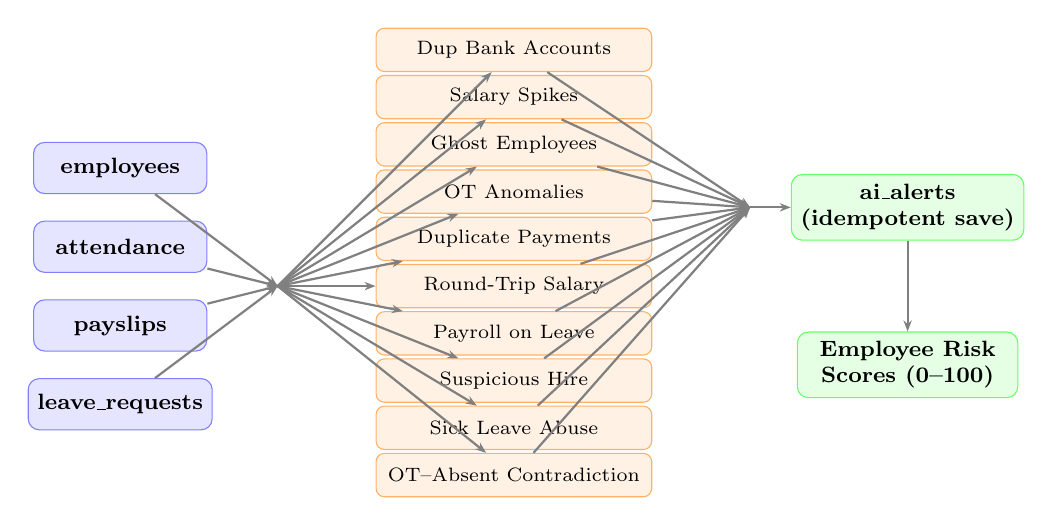
\begin{tikzpicture}[
  input/.style={rectangle, draw=blue!50, fill=blue!10, rounded corners=4pt, minimum width=2.2cm, minimum height=0.65cm, font=\footnotesize\bfseries, align=center},
  algo/.style={rectangle, draw=orange!60, fill=orange!10, rounded corners=3pt, minimum width=3.5cm, minimum height=0.55cm, font=\scriptsize, align=center},
  output/.style={rectangle, draw=green!60, fill=green!10, rounded corners=4pt, minimum width=2.8cm, minimum height=0.65cm, font=\footnotesize\bfseries, align=center},
  arr/.style={-{Stealth[length=4pt]}, draw=black!50, thick},
  node distance=0.4cm,
]
%% Inputs
\node[input] (emp)  at (0, 0)    {employees};
\node[input] (att)  at (0,-1)    {attendance};
\node[input] (pay)  at (0,-2)    {payslips};
\node[input] (lv)   at (0,-3)    {leave\_requests};

%% Algorithms (stacked)
\node[algo] (a1) at (5, 1.5)   {Dup Bank Accounts};
\node[algo] (a2) at (5, 0.9)   {Salary Spikes};
\node[algo] (a3) at (5, 0.3)   {Ghost Employees};
\node[algo] (a4) at (5,-0.3)   {OT Anomalies};
\node[algo] (a5) at (5,-0.9)   {Duplicate Payments};
\node[algo] (a6) at (5,-1.5)   {Round-Trip Salary};
\node[algo] (a7) at (5,-2.1)   {Payroll on Leave};
\node[algo] (a8) at (5,-2.7)   {Suspicious Hire};
\node[algo] (a9) at (5,-3.3)   {Sick Leave Abuse};
\node[algo] (a10) at (5,-3.9)  {OT--Absent Contradiction};

%% Outputs
\node[output] (alerts)  at (10,-0.5) {ai\_alerts\\(idempotent save)};
\node[output] (risk)    at (10,-2.5) {Employee Risk\\Scores (0--100)};

%% Input to algorithms
\foreach \a in {a1,a2,a3,a4,a5,a6,a7,a8,a9,a10} {
  \draw[arr] (2, -1.5) -- (\a);
}
\draw[arr] (emp) -- (2,-1.5);
\draw[arr] (att) -- (2,-1.5);
\draw[arr] (pay) -- (2,-1.5);
\draw[arr] (lv)  -- (2,-1.5);

%% Algorithms to outputs
\foreach \a in {a1,a2,a3,a4,a5,a6,a7,a8,a9,a10} {
  \draw[arr] (\a) -- (8,-0.5);
}
\draw[arr] (8,-0.5) -- (alerts);
\draw[arr] (alerts) -- (risk);
\end{tikzpicture}
\caption{Fraud Detection Pipeline --- Inputs, 10 Algorithms, and Outputs}
\label{fig:fraud_pipeline}
\end{figure}

\subsubsection{Employee Risk Scoring}

Each employee receives a risk score (0--100) computed as:
\[
\text{Score} = \min\!\left(100,\; \sum_{\text{alert}} w_\text{sev} \times \frac{\text{confidence}}{100} \times r_\text{recency}\right)
\]
where severity weights are: critical = 40, high = 25, medium = 12, low = 5; and recency factors are: $\leq$30 days = 1.0, $\leq$60 days = 0.7, older = 0.4. Risk tiers: 0--24 Low, 25--49 Medium, 50--74 High, 75--100 Critical.

\subsubsection{Alert Case Management Workflow}

Alerts persisted in \texttt{ai\_alerts} follow the status lifecycle shown in Figure~\ref{fig:alert_workflow}.

\begin{figure}[H]
\centering
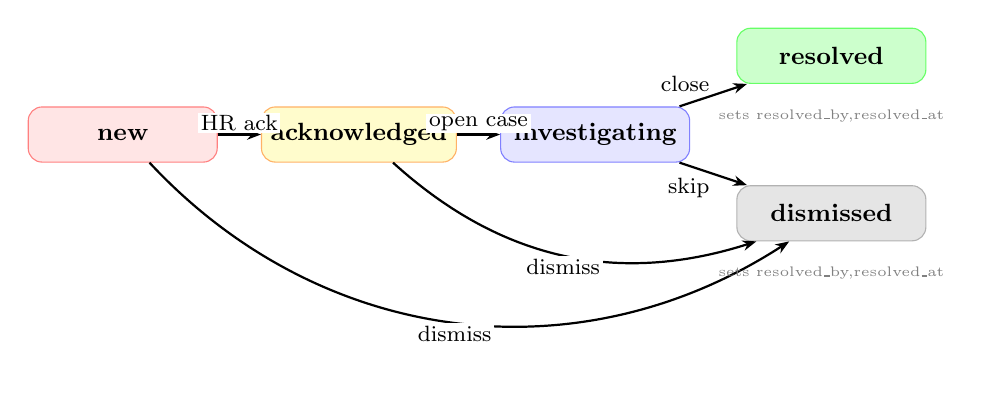
\begin{tikzpicture}[
  st/.style={rectangle, rounded corners=5pt, draw=black!50, fill=white, minimum width=2.4cm, minimum height=0.7cm, font=\small\bfseries, align=center},
  newst/.style={st, fill=red!10, draw=red!50},
  ackst/.style={st, fill=yellow!20, draw=orange!60},
  invst/.style={st, fill=blue!10, draw=blue!50},
  resst/.style={st, fill=green!20, draw=green!60},
  disst/.style={st, fill=gray!20, draw=gray!60},
  arr/.style={-{Stealth[length=5pt]}, thick},
  lbl/.style={font=\footnotesize, fill=white, inner sep=1pt},
]
\node[newst] (new)  at (0,0)    {new};
\node[ackst] (ack)  at (3,0)    {acknowledged};
\node[invst] (inv)  at (6,0)    {investigating};
\node[resst] (res)  at (9, 1)   {resolved};
\node[disst] (dis)  at (9,-1)   {dismissed};

\draw[arr] (new)  -- node[lbl,above]{HR ack}    (ack);
\draw[arr] (ack)  -- node[lbl,above]{open case} (inv);
\draw[arr] (inv)  -- node[lbl,above left]{close} (res);
\draw[arr] (inv)  -- node[lbl,below left]{skip}  (dis);
\draw[arr] (new)  to[bend right=40] node[lbl,below]{dismiss} (dis);
\draw[arr] (ack)  to[bend right=30] node[lbl,below]{dismiss} (dis);

\node[font=\tiny, text=gray, below=0.2cm of res] {sets resolved\_by,\\resolved\_at};
\node[font=\tiny, text=gray, below=0.2cm of dis] {sets resolved\_by,\\resolved\_at};
\end{tikzpicture}
\caption{AI Alert Case Management Status Lifecycle}
\label{fig:alert_workflow}
\end{figure}

\textbf{HR Chatbot (\texttt{chatbot.service.js}):}

The chatbot uses intent classification to match user queries to predefined intent handlers. Supported intents include salary queries, leave balance enquiries, attendance status, and general HR information.

Figure~\ref{fig:chatbot_intent} shows the intent classification flowchart used by the chatbot service.

\begin{figure}[H]
\centering
\begin{tikzpicture}[
  proc/.style={rectangle, draw=purple!50, fill=purple!8, rounded corners=3pt, minimum width=4.2cm, minimum height=0.65cm, font=\small, align=center},
  dec/.style={diamond, draw=orange!60, fill=orange!10, font=\scriptsize, align=center, aspect=3},
  out/.style={rectangle, draw=teal!60, fill=teal!10, rounded corners=4pt, minimum width=3.5cm, minimum height=0.6cm, font=\footnotesize\ttfamily, align=center},
  term/.style={rectangle, draw=green!60, fill=green!12, rounded corners=8pt, minimum width=4.2cm, minimum height=0.6cm, font=\small\bfseries},
  arr/.style={-{Stealth[length=4pt]}, thick},
  lbl/.style={font=\footnotesize, fill=white, inner sep=1pt},
  node distance=0.55cm,
]
\node[term]  (start) at (0,0)    {User message received};
\node[proc]  (lower) at (0,-1.2) {Normalise: lowercase};
\node[dec]   (d1)    at (0,-2.5) {salary/pay/\\payslip?};
\node[dec]   (d2)    at (0,-4.0) {leave balance/\\remaining?};
\node[dec]   (d3)    at (0,-5.5) {attendance/\\check-in?};
\node[dec]   (d4)    at (0,-7.0) {tax/fbr/eobi?};
\node[dec]   (d5)    at (0,-8.5) {policy/holiday?};

\node[out] (r1) at (5.5,-2.5) {SALARY\_QUERY};
\node[out] (r2) at (5.5,-4.0) {LEAVE\_BALANCE};
\node[out] (r3) at (5.5,-5.5) {ATTENDANCE\_STATUS};
\node[out] (r4) at (5.5,-7.0) {TAX\_INFO};
\node[out] (r5) at (5.5,-8.5) {HR\_POLICY};
\node[out] (r6) at (5.5,-9.7) {GENERAL};

\draw[arr] (start) -- (lower);
\draw[arr] (lower) -- (d1);
\draw[arr] (d1)  -- node[lbl,above]{yes} (r1);
\draw[arr] (d1)  -- node[lbl,right]{no}  (d2);
\draw[arr] (d2)  -- node[lbl,above]{yes} (r2);
\draw[arr] (d2)  -- node[lbl,right]{no}  (d3);
\draw[arr] (d3)  -- node[lbl,above]{yes} (r3);
\draw[arr] (d3)  -- node[lbl,right]{no}  (d4);
\draw[arr] (d4)  -- node[lbl,above]{yes} (r4);
\draw[arr] (d4)  -- node[lbl,right]{no}  (d5);
\draw[arr] (d5)  -- node[lbl,above]{yes} (r5);
\draw[arr] (d5.east) -- ++(0.6,0) |- node[lbl,right]{no} (r6);
\end{tikzpicture}
\caption{HR Chatbot Intent Classification Flowchart}
\label{fig:chatbot_intent}
\end{figure}

\subsection{Stage 6: Frontend Development}

The React frontend was built with the following technology choices:

\begin{itemize}
    \item \textbf{React 18.3.1} with functional components and hooks
    \item \textbf{TypeScript 5.8.3} for compile-time type safety
    \item \textbf{TanStack Query 5.83.0} for server state management and caching
    \item \textbf{Redux Toolkit 2.11.2} for client-side session state
    \item \textbf{Tailwind CSS 3.4.17} with shadcn/ui components (Radix UI primitives)
    \item \textbf{Axios 1.13.4} for HTTP requests with JWT interceptor and auto-refresh
    \item \textbf{Recharts 2.15.4} for analytics charts on the AI Insights page
    \item \textbf{Vite 5.4.19} as the build tool
\end{itemize}

All API calls are encapsulated in custom hooks (\texttt{useAuth}, \texttt{useEmployees}, \texttt{useAttendance}, \texttt{useLeaves}, \texttt{usePayroll}, \texttt{useAI}, \texttt{useNotifications}). Each hook uses \texttt{useQuery} for read operations and \texttt{useMutation} for write operations, providing automatic caching, background refetching, and loading/error state management.

\section{User Interface}

The frontend provides role-specific dashboards and feature pages. Figure~\ref{fig:hr_dashboard} shows the HR dashboard, which is the primary landing page for HR administrators.

\begin{figure}[H]
\centering
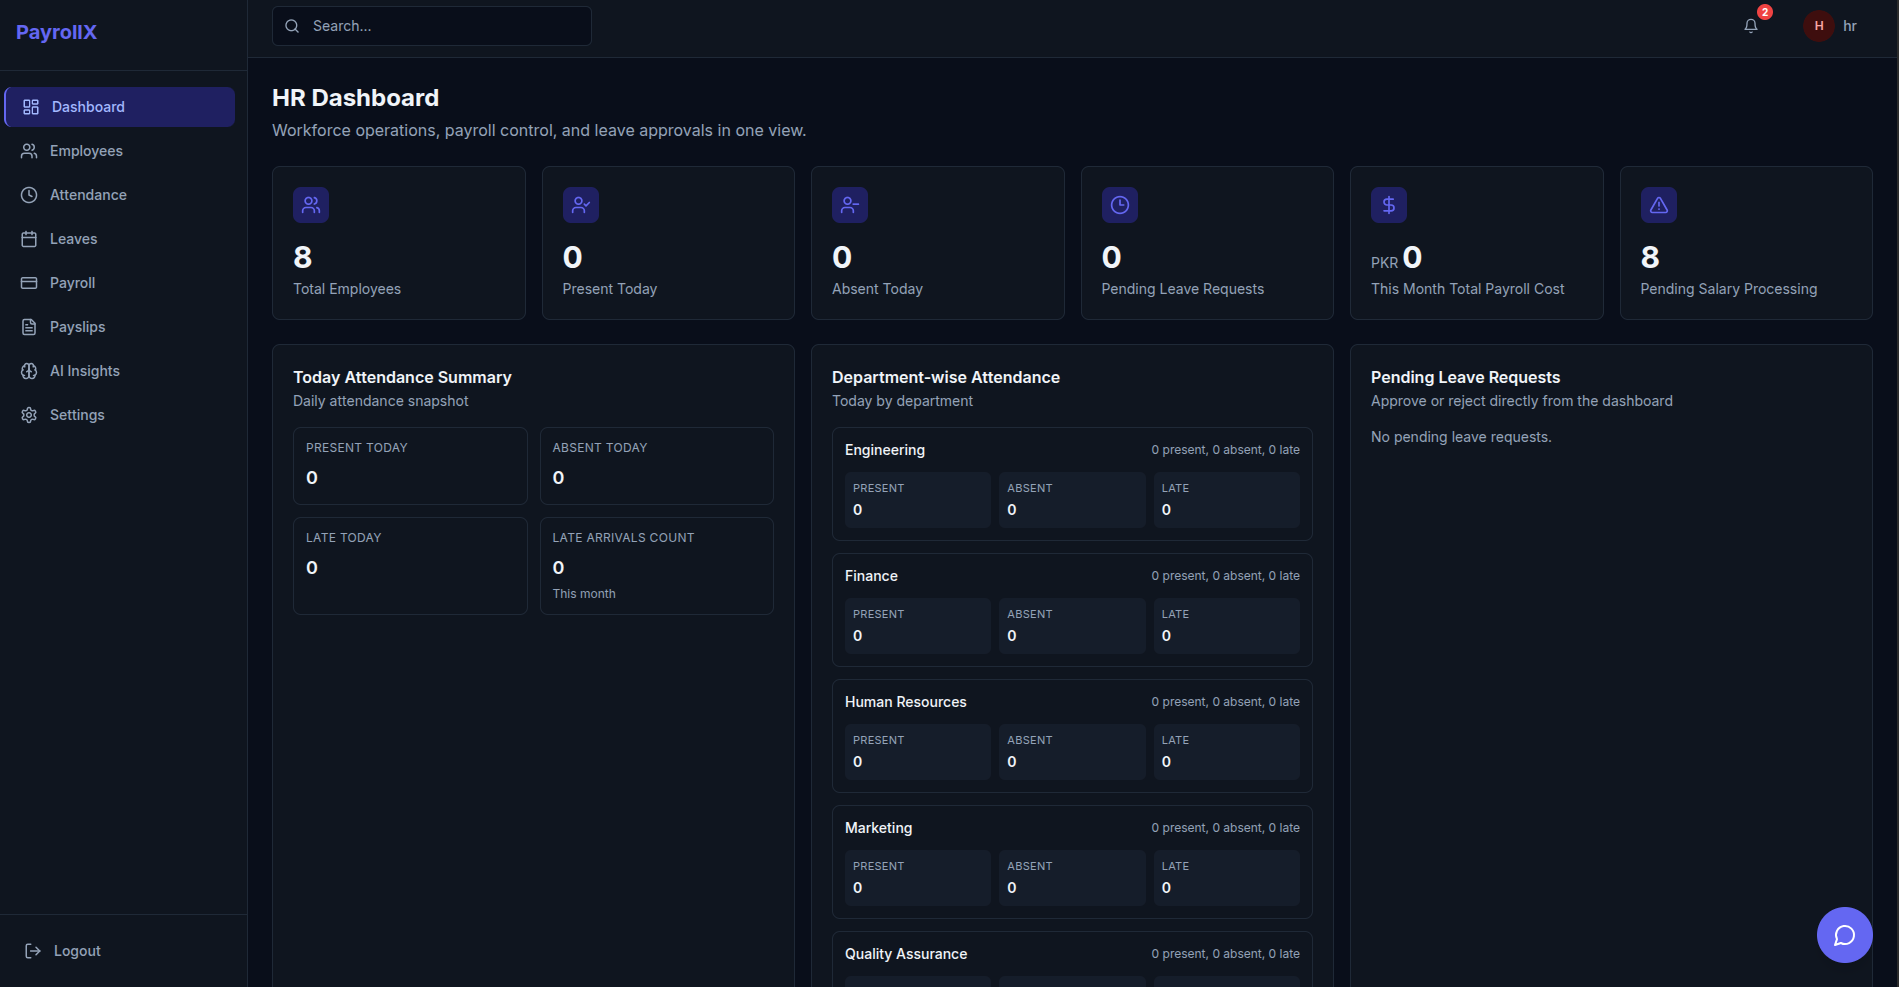
\includegraphics[width=0.95\textwidth]{media/hr dashboard.png}
\caption{HR Dashboard --- Summary Cards, Attendance Stats, and Quick Actions}
\label{fig:hr_dashboard}
\end{figure}

\subsection{Employee Management}

Figure~\ref{fig:hr_employees} shows the HR employee list page, which displays all employees with search and filter capabilities. HR can view department, designation, and employment status at a glance.

\begin{figure}[H]
\centering
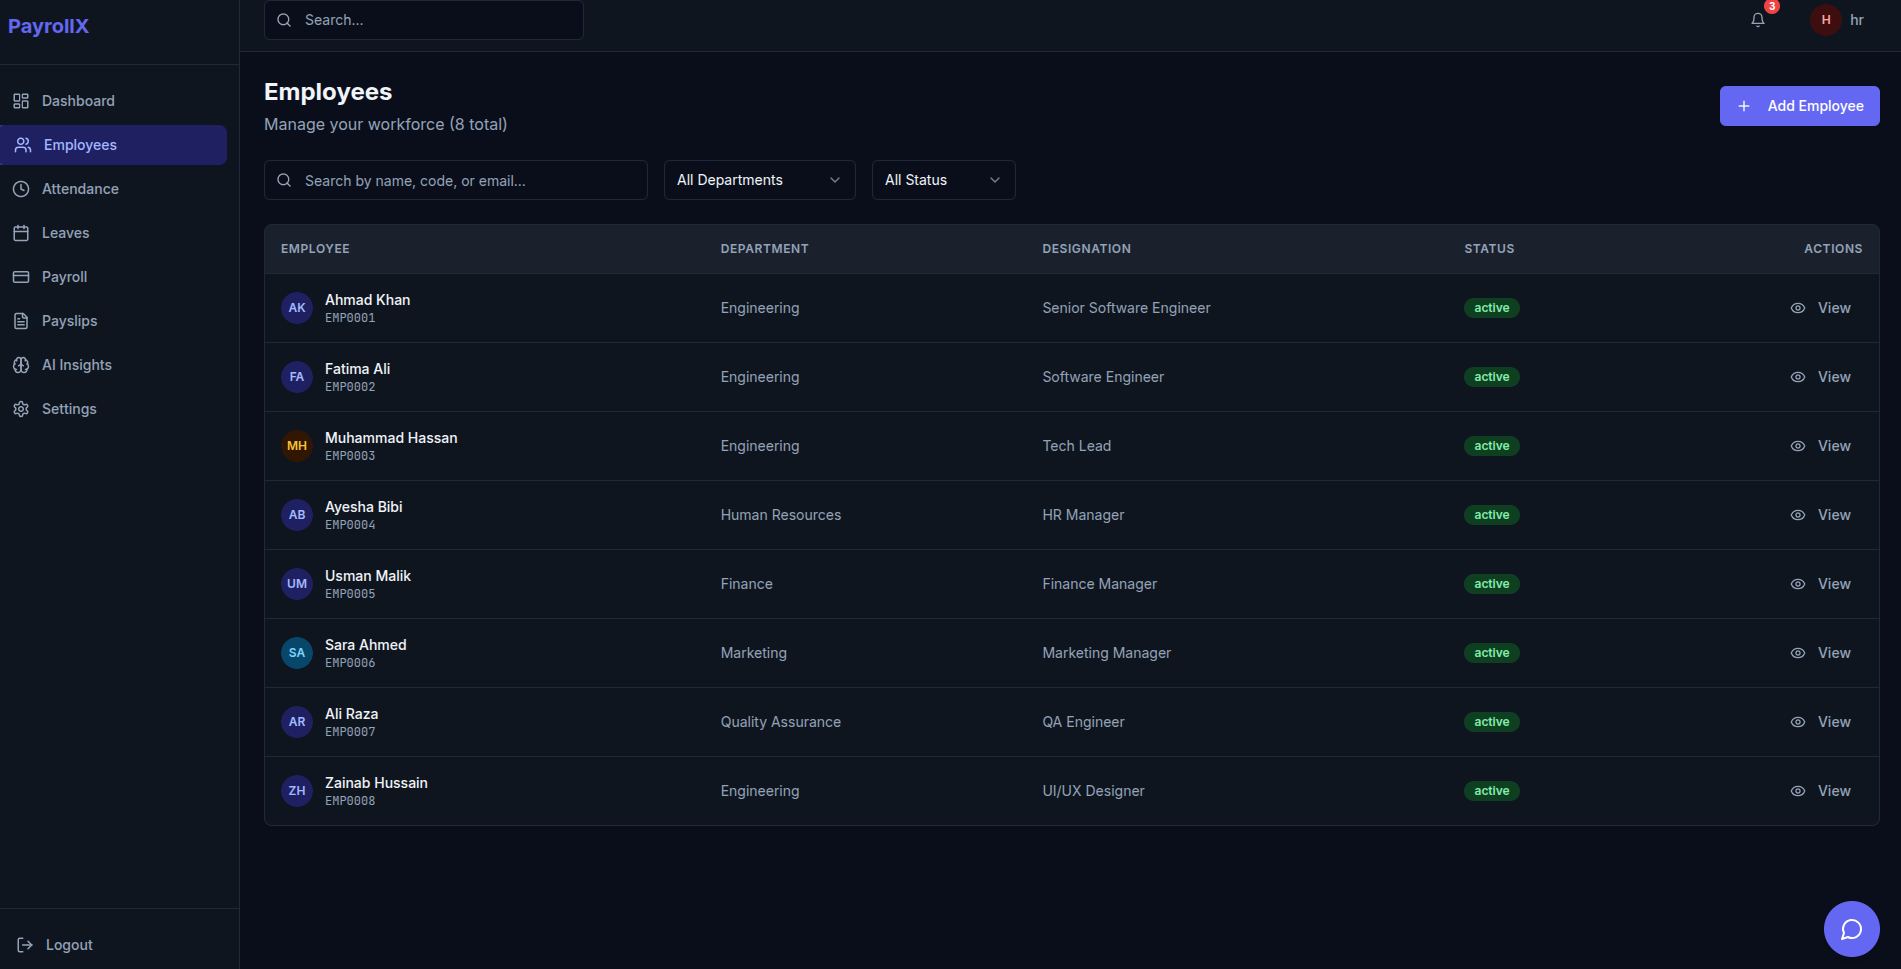
\includegraphics[width=0.95\textwidth]{media/hr employees.png}
\caption{HR Employee List --- Searchable, Filterable Employee Directory}
\label{fig:hr_employees}
\end{figure}

Figure~\ref{fig:add_employee} shows the Add Employee form, which collects all required fields including personal information, department assignment, designation, salary details, and bank account information.

\begin{figure}[H]
\centering
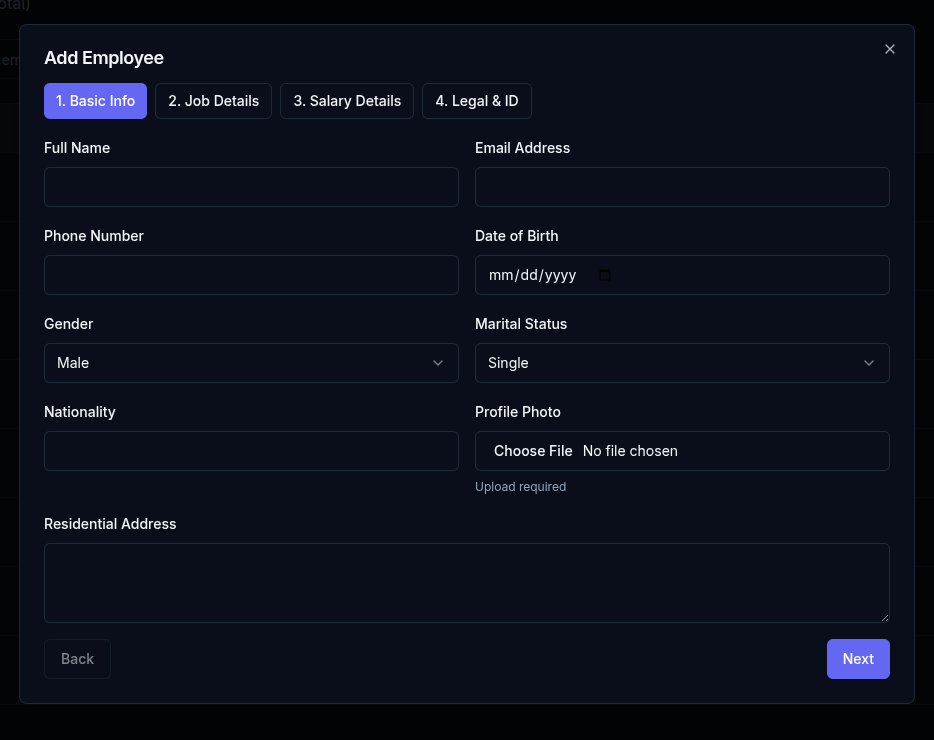
\includegraphics[width=0.95\textwidth]{media/add employee.png}
\caption{Add Employee Form --- Complete Employee Onboarding Interface}
\label{fig:add_employee}
\end{figure}

\subsection{Attendance Management}

Figure~\ref{fig:hr_attendance} shows the HR attendance view, where administrators can see daily attendance records across all employees, mark attendance manually, and view summary statistics.

\begin{figure}[H]
\centering
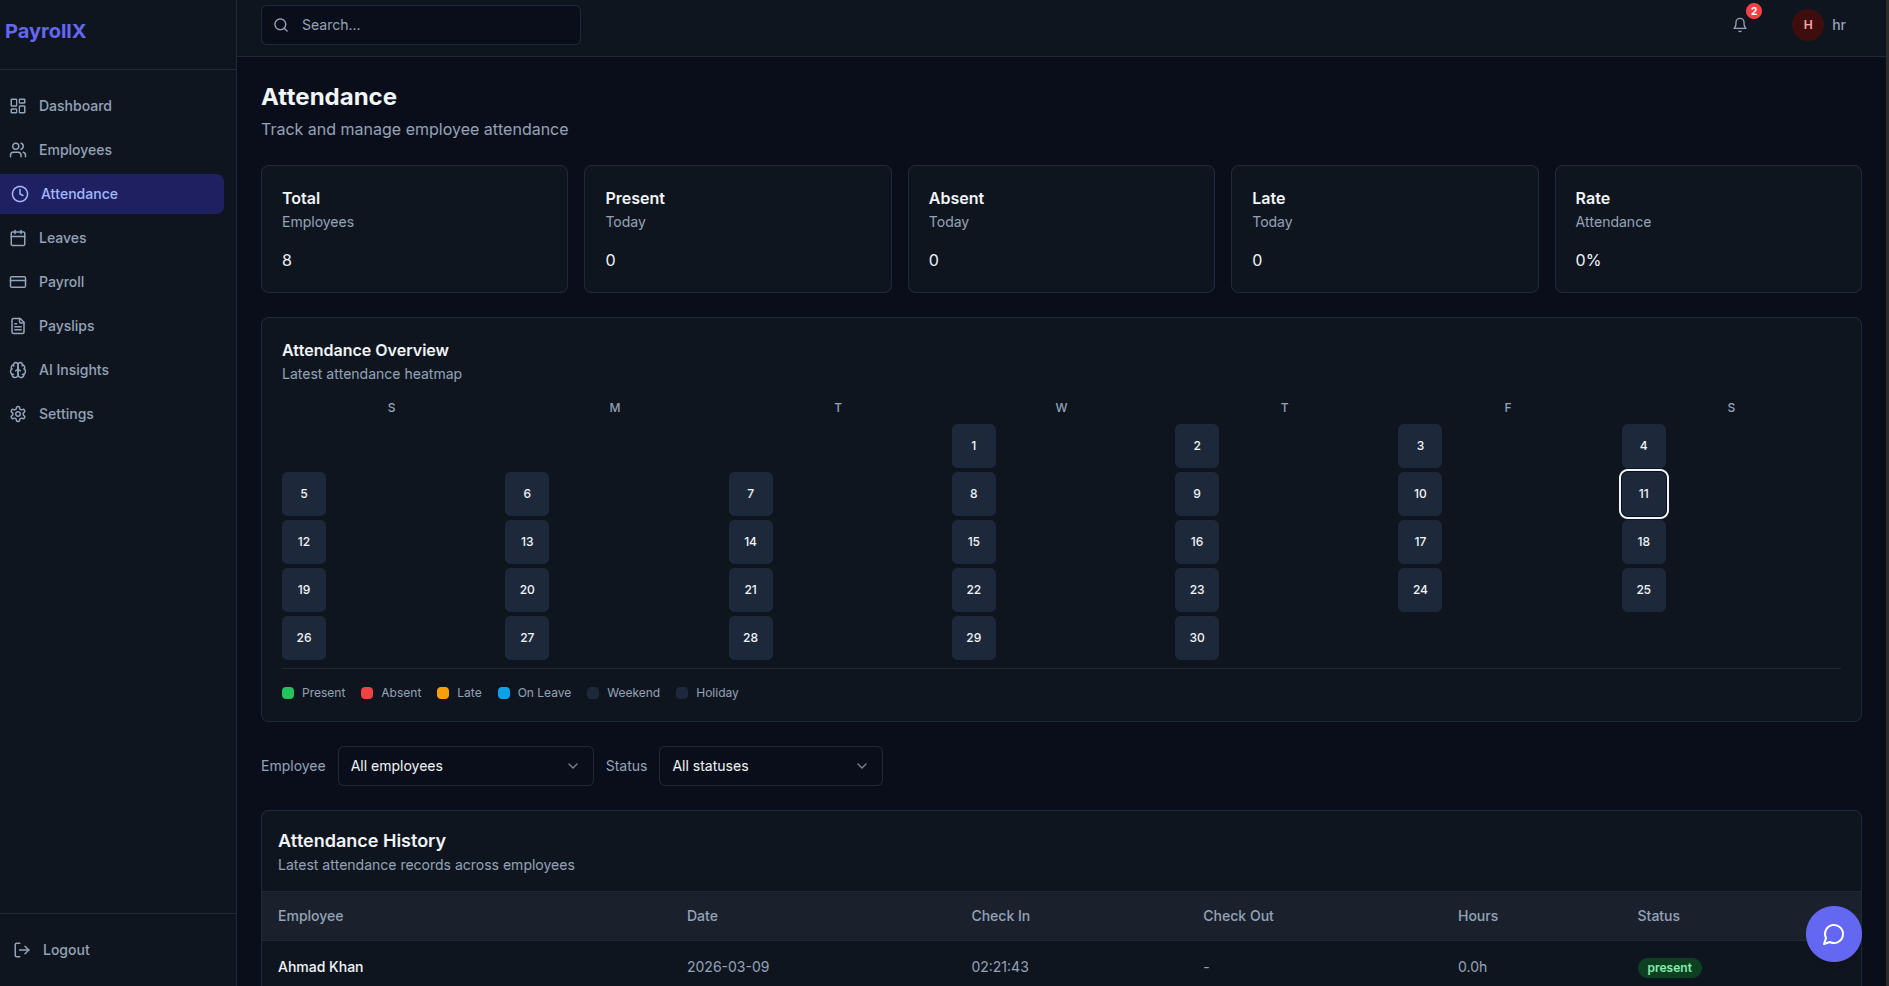
\includegraphics[width=0.95\textwidth]{media/hr attandance.png}
\caption{HR Attendance Management --- Daily Records and Manual Marking}
\label{fig:hr_attendance}
\end{figure}

Figure~\ref{fig:emp_attendance} shows the employee attendance page, where employees can check in, check out, and review their own attendance history.

\begin{figure}[H]
\centering
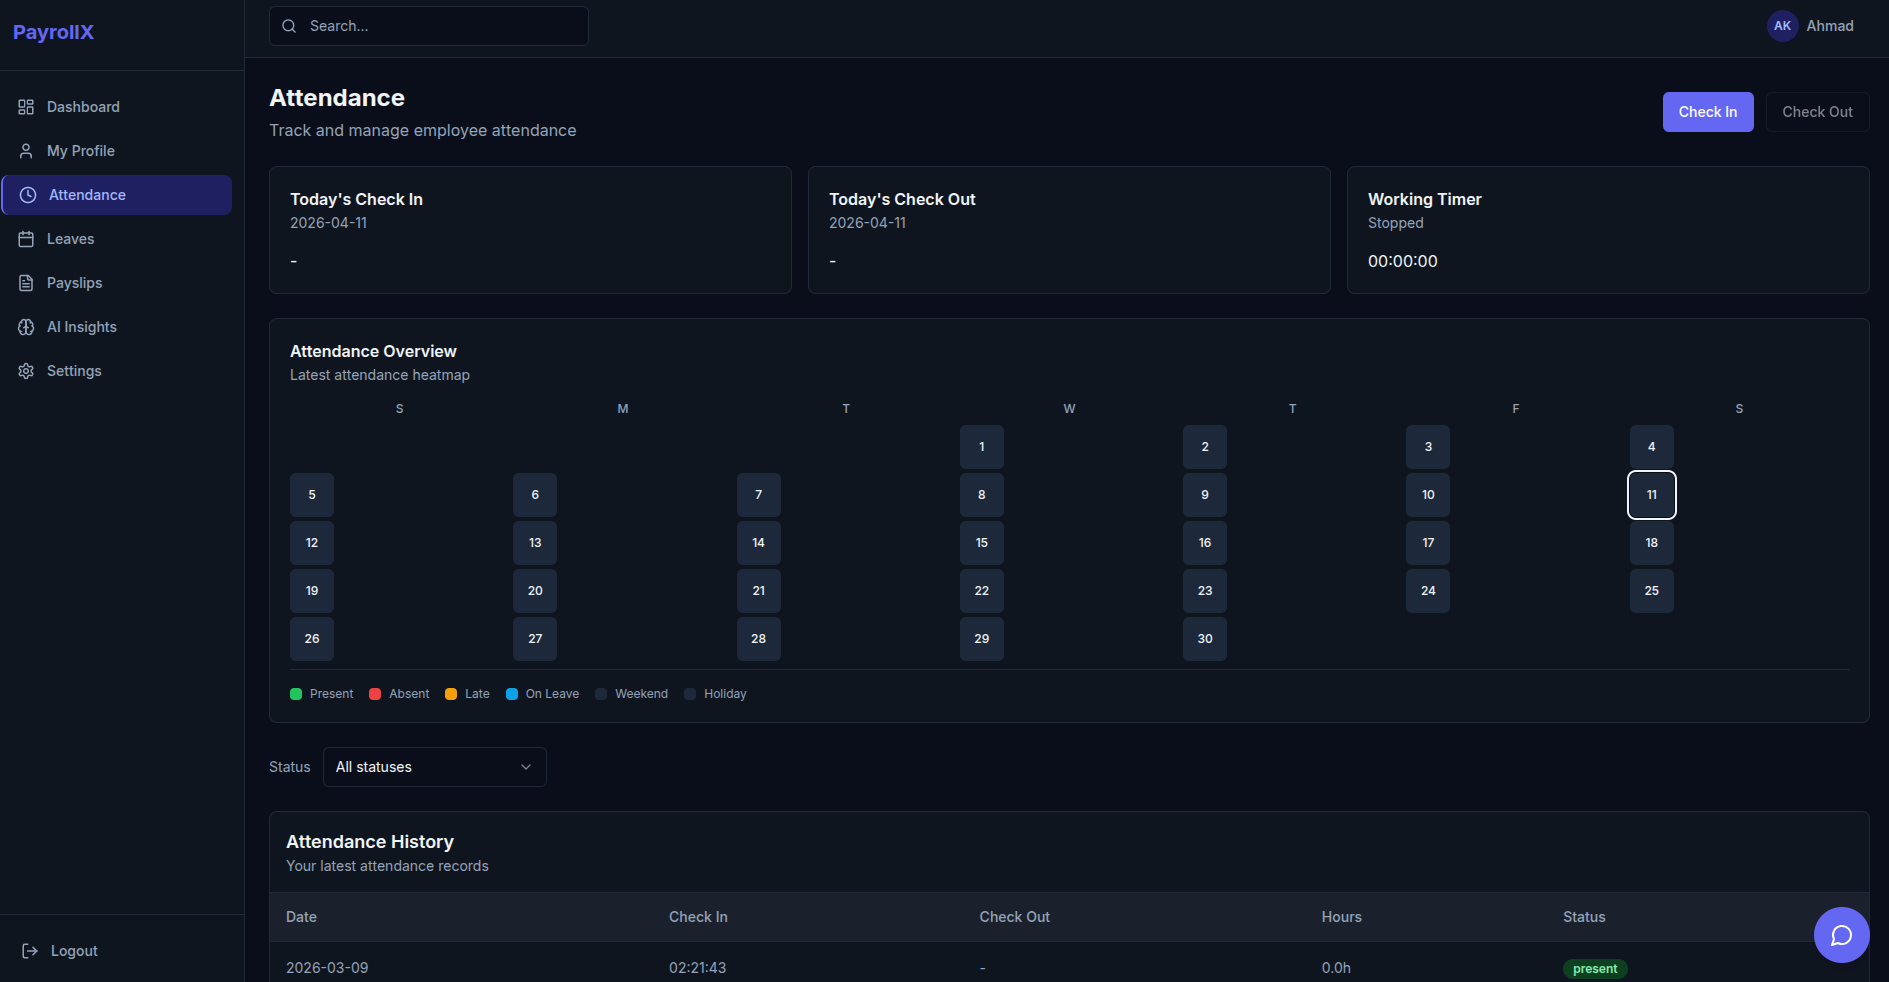
\includegraphics[width=0.95\textwidth]{media/attandance.png}
\caption{Employee Attendance Page --- Check-In/Out and Personal History}
\label{fig:emp_attendance}
\end{figure}

\subsection{Leave Management}

Figure~\ref{fig:leaves} shows the leave management page as seen by an employee, with the leave request submission form and the list of current and past leave applications with their status.

\begin{figure}[H]
\centering
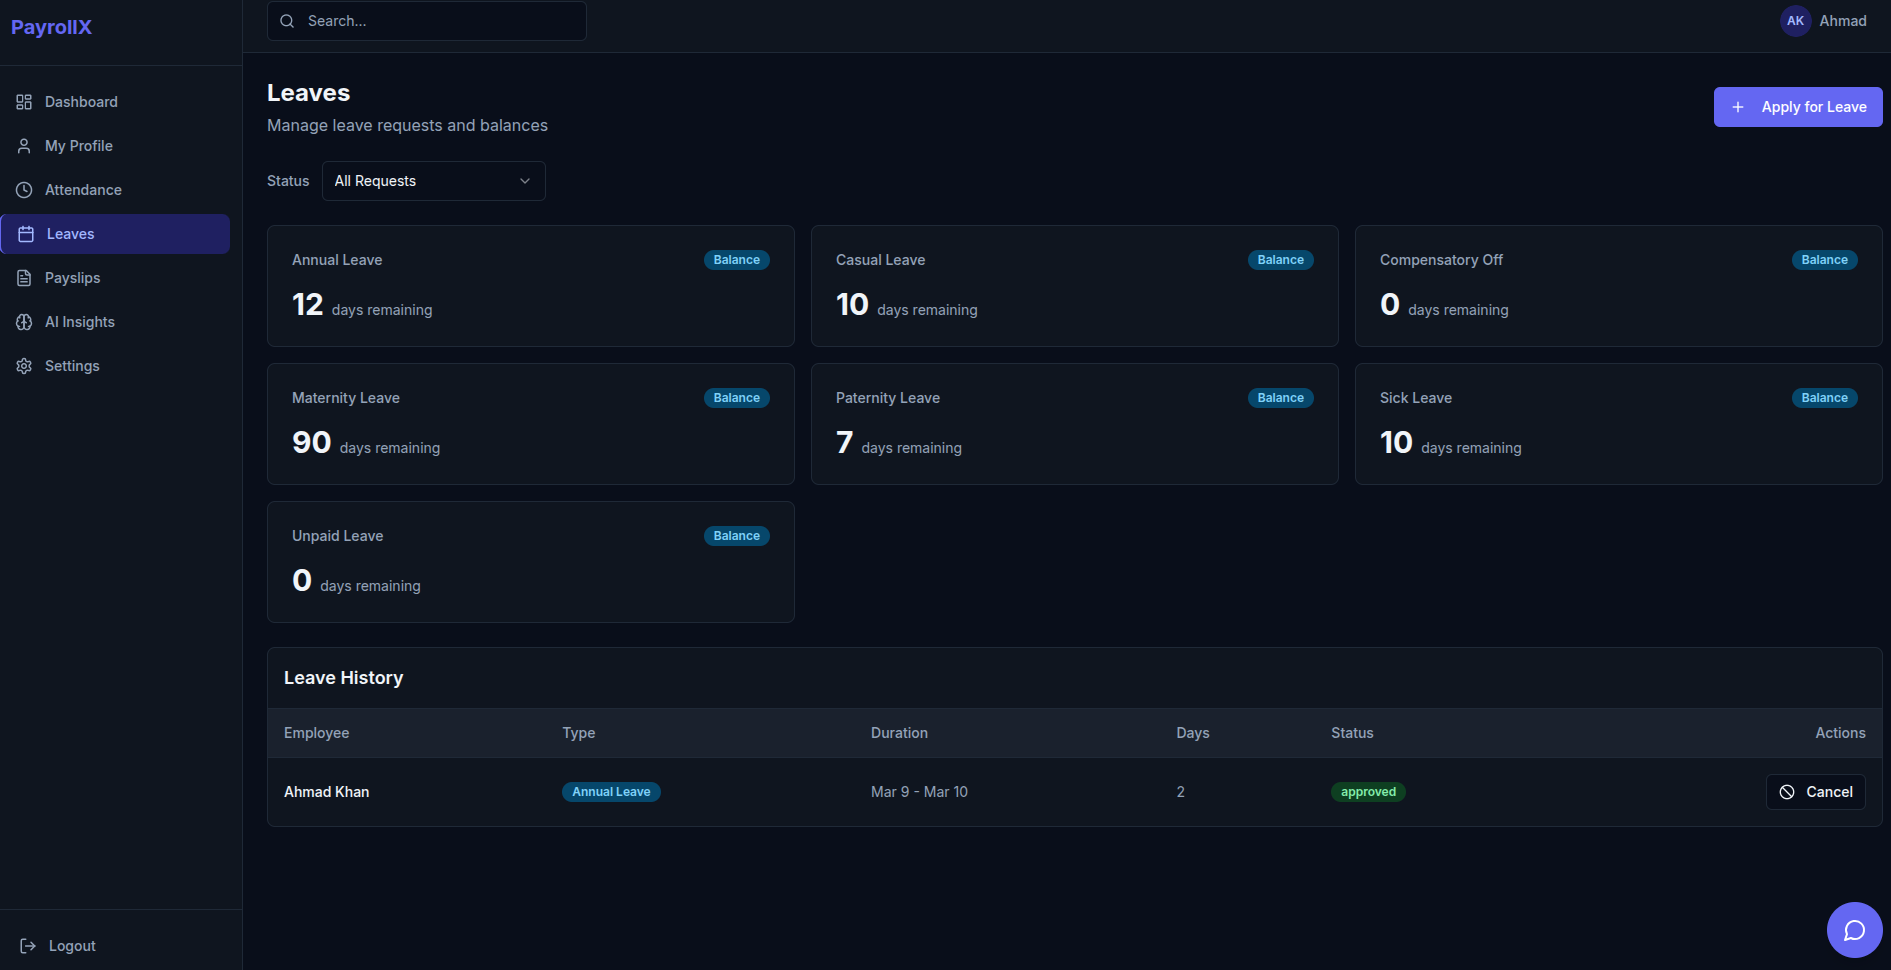
\includegraphics[width=0.95\textwidth]{media/leaves.png}
\caption{Leave Management Page --- Request Submission and Application History}
\label{fig:leaves}
\end{figure}

Figure~\ref{fig:leave_balance} shows the leave balance summary, displaying remaining entitlement per leave type for the current year.

\begin{figure}[H]
\centering
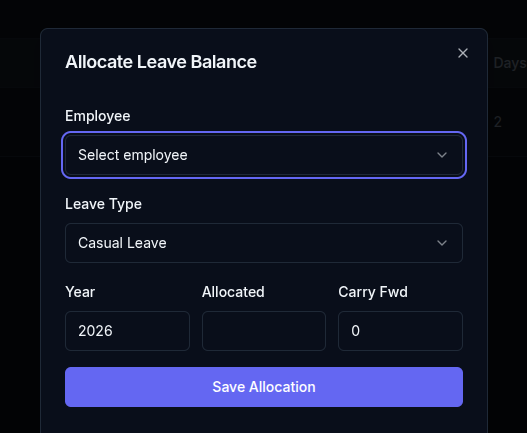
\includegraphics[width=0.95\textwidth]{media/leave balance.png}
\caption{Leave Balance Summary --- Remaining Entitlement per Leave Type}
\label{fig:leave_balance}
\end{figure}

\subsection{Payroll and Payslips}

Figure~\ref{fig:hr_payslips} shows the HR payroll management page, where administrators can initiate payroll runs, monitor processing status, and access payslip records for all employees.

\begin{figure}[H]
\centering
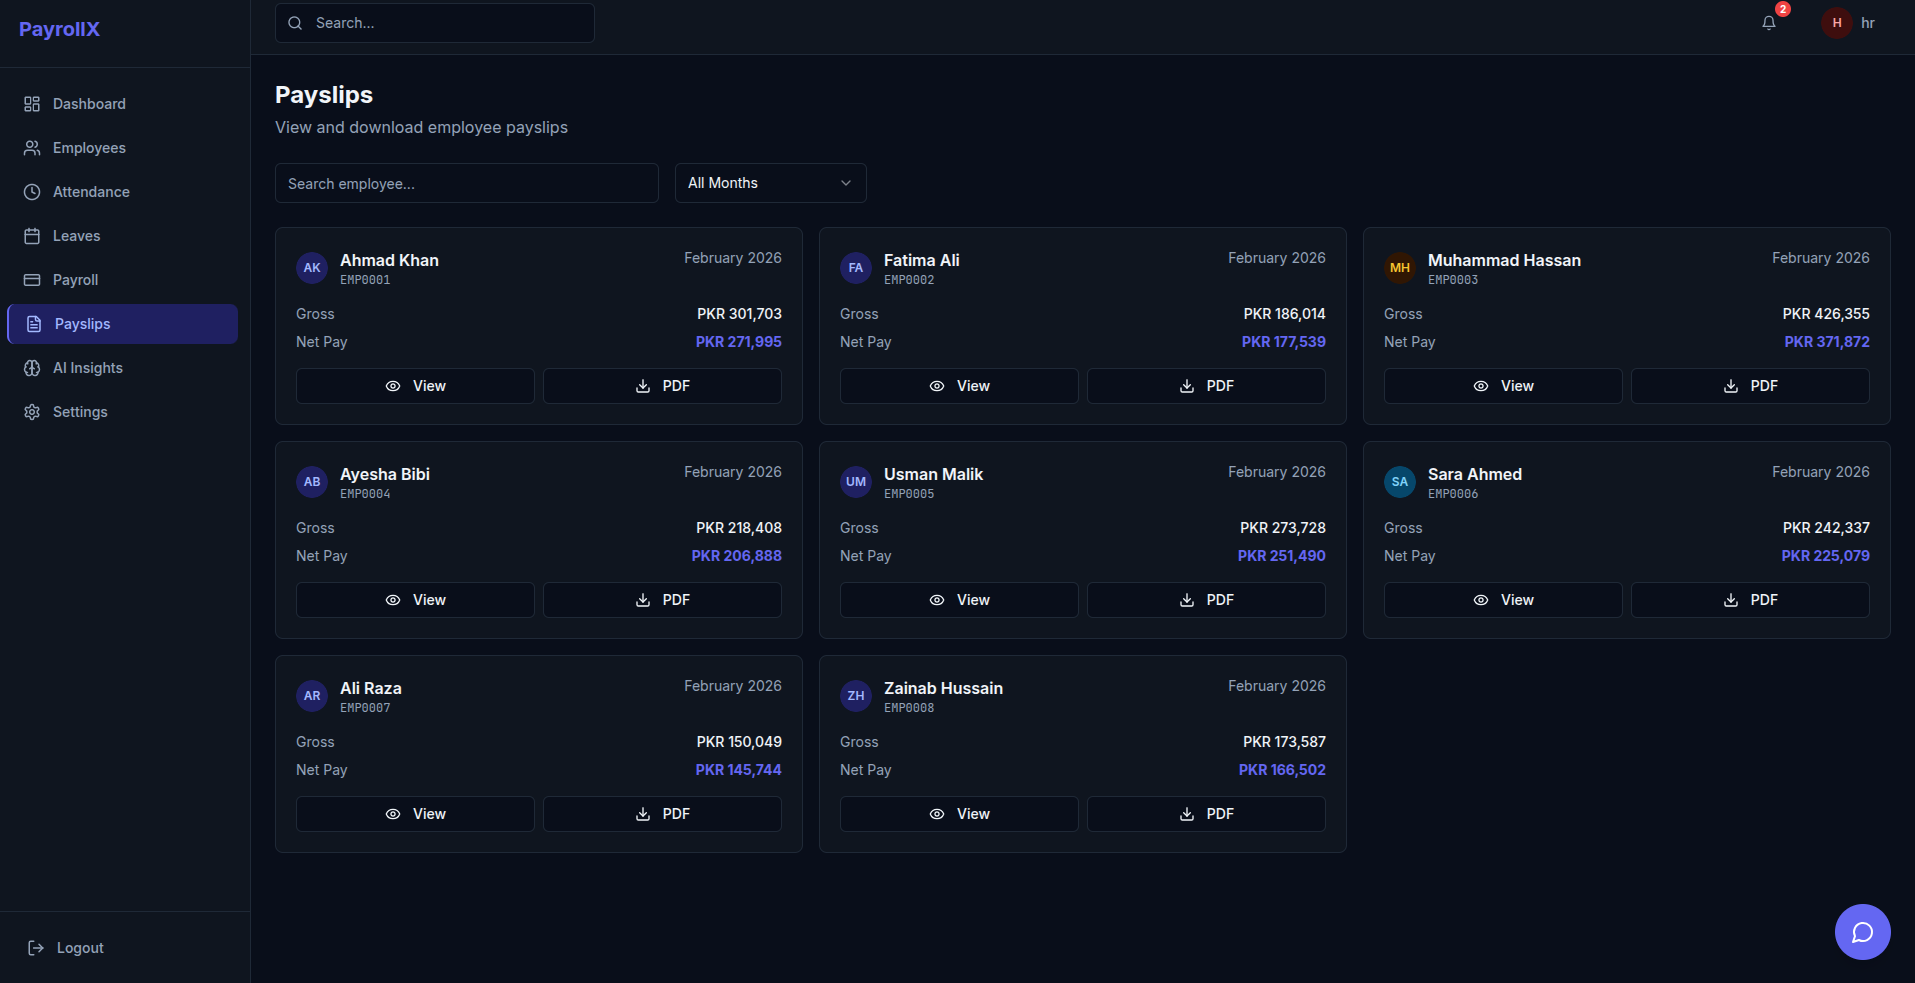
\includegraphics[width=0.95\textwidth]{media/hr payslips.png}
\caption{HR Payroll Management --- Run Initiation, Status, and Payslip Records}
\label{fig:hr_payslips}
\end{figure}

Figure~\ref{fig:payslips} shows the employee payslips page, where employees can browse their payslip history and download individual payslips.

\begin{figure}[H]
\centering
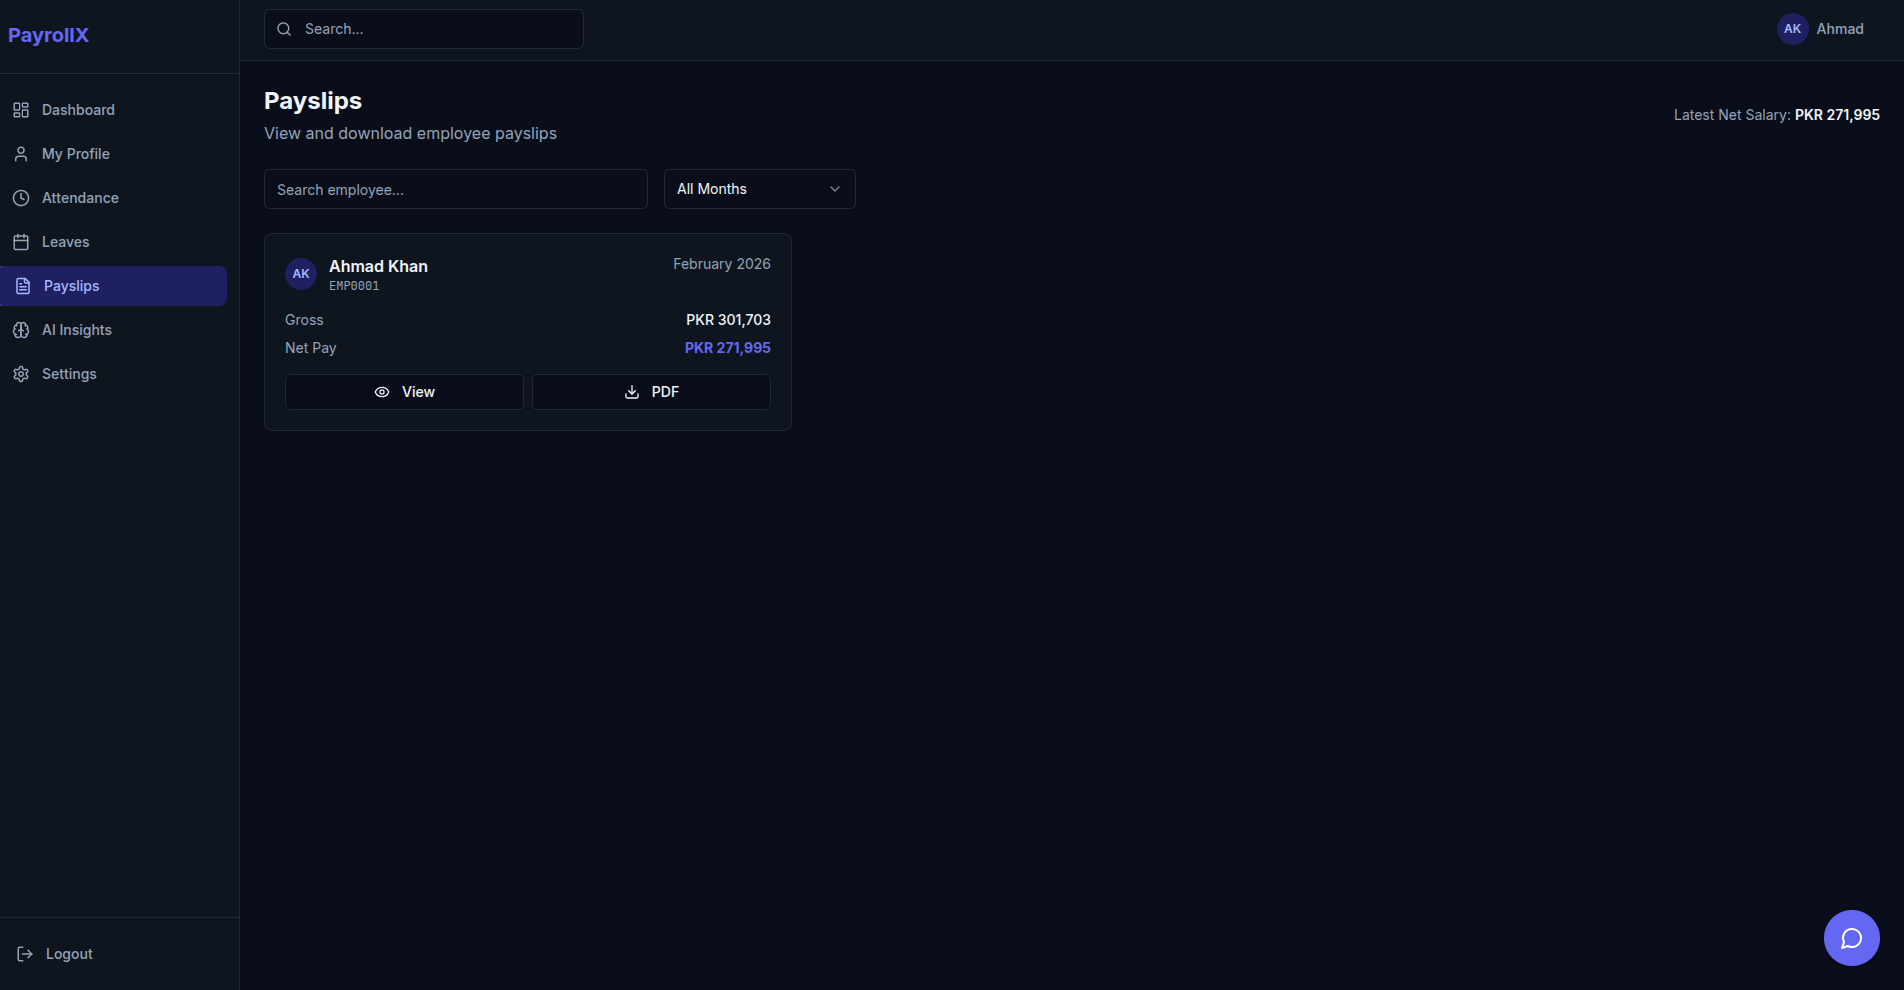
\includegraphics[width=0.95\textwidth]{media/payslips.png}
\caption{Employee Payslips Page --- Payslip History and Download}
\label{fig:payslips}
\end{figure}

\subsection{AI Insights and Chatbot}

Figure~\ref{fig:insights} shows the AI Insights page, which aggregates outputs from all five AI modules: fraud detection alerts, salary anomaly findings, payroll forecasts, salary recommendations, and chatbot access.

\begin{figure}[H]
\centering
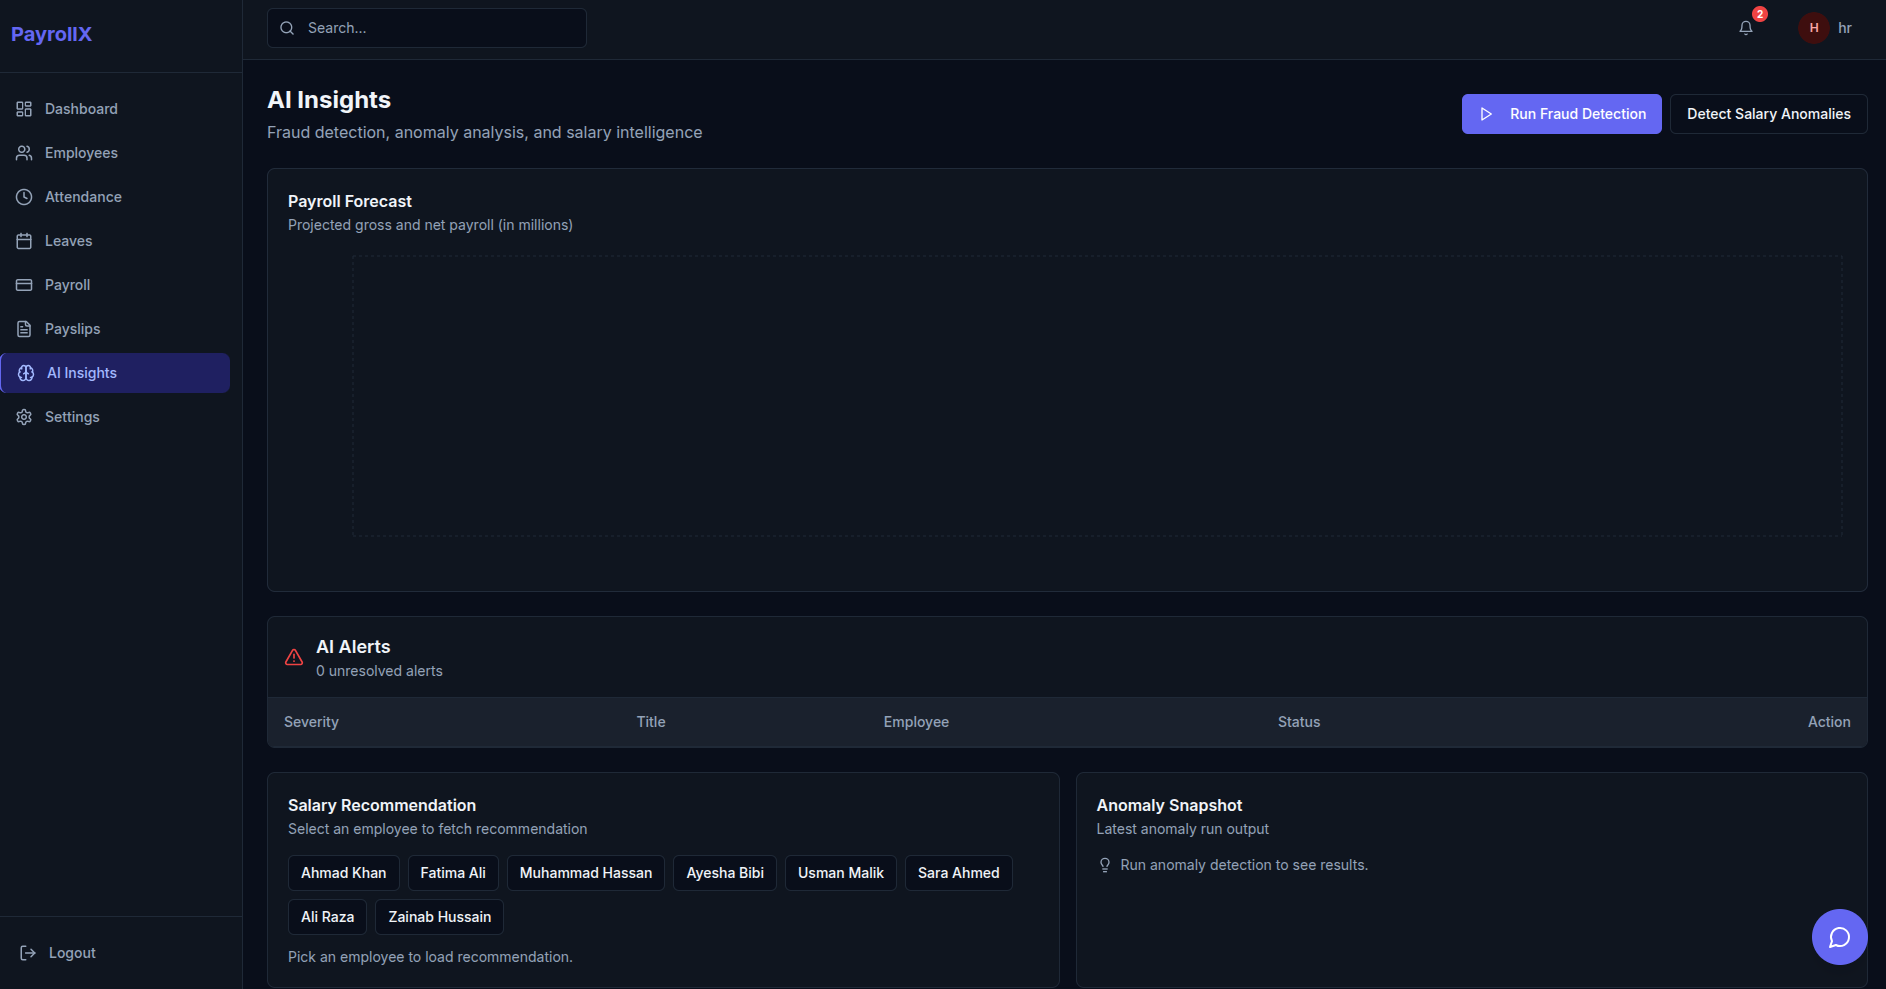
\includegraphics[width=0.95\textwidth]{media/insights.png}
\caption{AI Insights Dashboard --- Fraud Alerts, Anomaly Detection, and Forecasts}
\label{fig:insights}
\end{figure}

Figure~\ref{fig:chatbot} shows the HR chatbot interface. Employees type natural language queries and receive contextually relevant responses drawn from their own employee data (salary, leave balances, attendance status).

\begin{figure}[H]
\centering
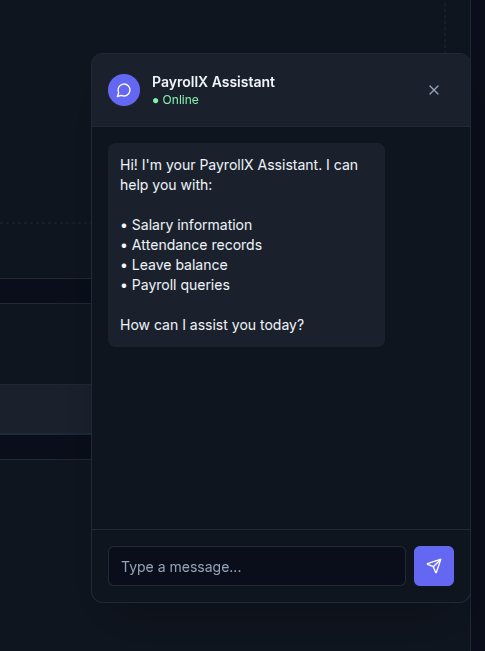
\includegraphics[width=0.95\textwidth]{media/chatboart.png}
\caption{HR Chatbot --- Intent-Based Natural Language Interface for Employee Queries}
\label{fig:chatbot}
\end{figure}

\subsection{Self-Service Profile and Notifications}

Figure~\ref{fig:profile} shows the employee self-service profile page, where employees can view their personal details, employment information, and payslip history without contacting HR.

\begin{figure}[H]
\centering
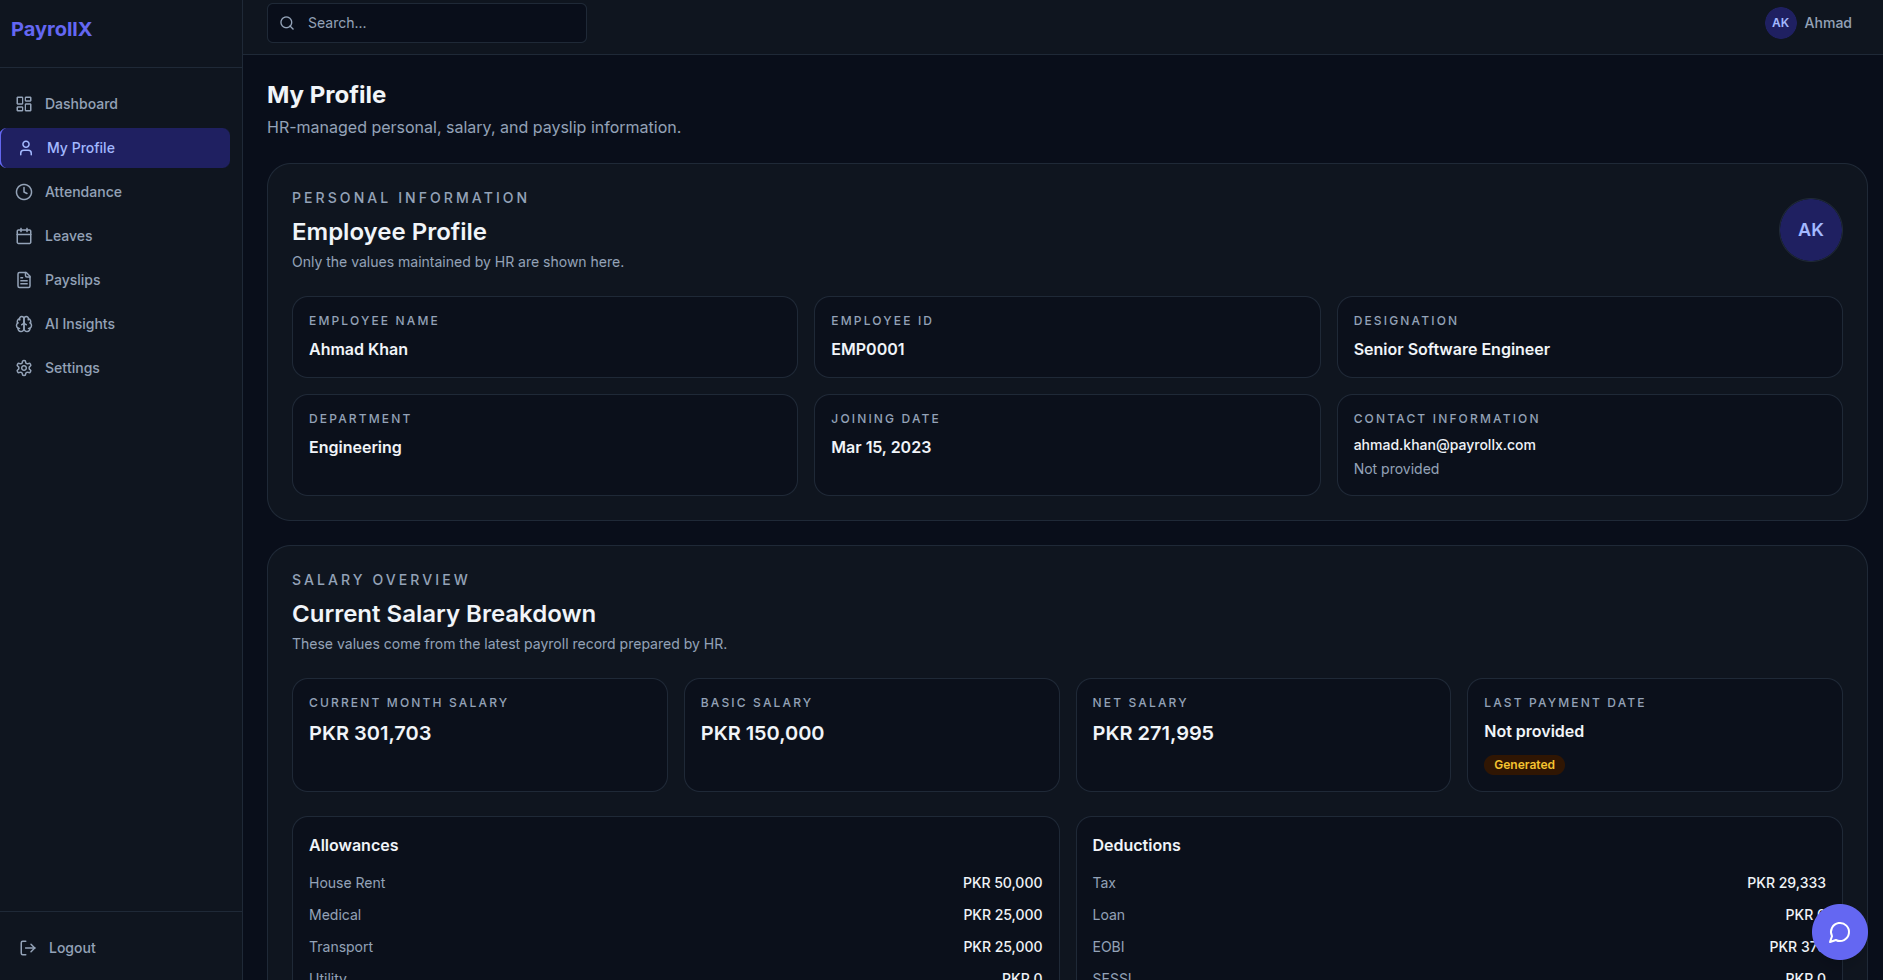
\includegraphics[width=0.95\textwidth]{media/profile.png}
\caption{Employee Self-Service Profile --- Personal Details, Employment Info, and Payslips}
\label{fig:profile}
\end{figure}

Figure~\ref{fig:notifications} shows the notifications centre, where employees can see all in-app notifications including leave status changes, salary credits, and company notices, with an unread badge count.

\begin{figure}[H]
\centering
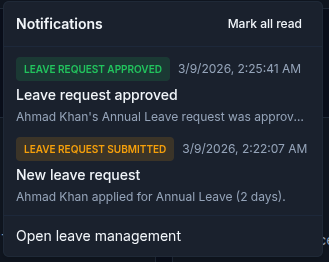
\includegraphics[width=0.95\textwidth]{media/notificatios.png}
\caption{Notifications Centre --- In-App Alerts for Leave Status and Salary Events}
\label{fig:notifications}
\end{figure}

\subsection{System Settings}

Figure~\ref{fig:settings} shows the system settings page, accessible to HR administrators, where public holidays, tax configuration, and system preferences can be managed.

\begin{figure}[H]
\centering
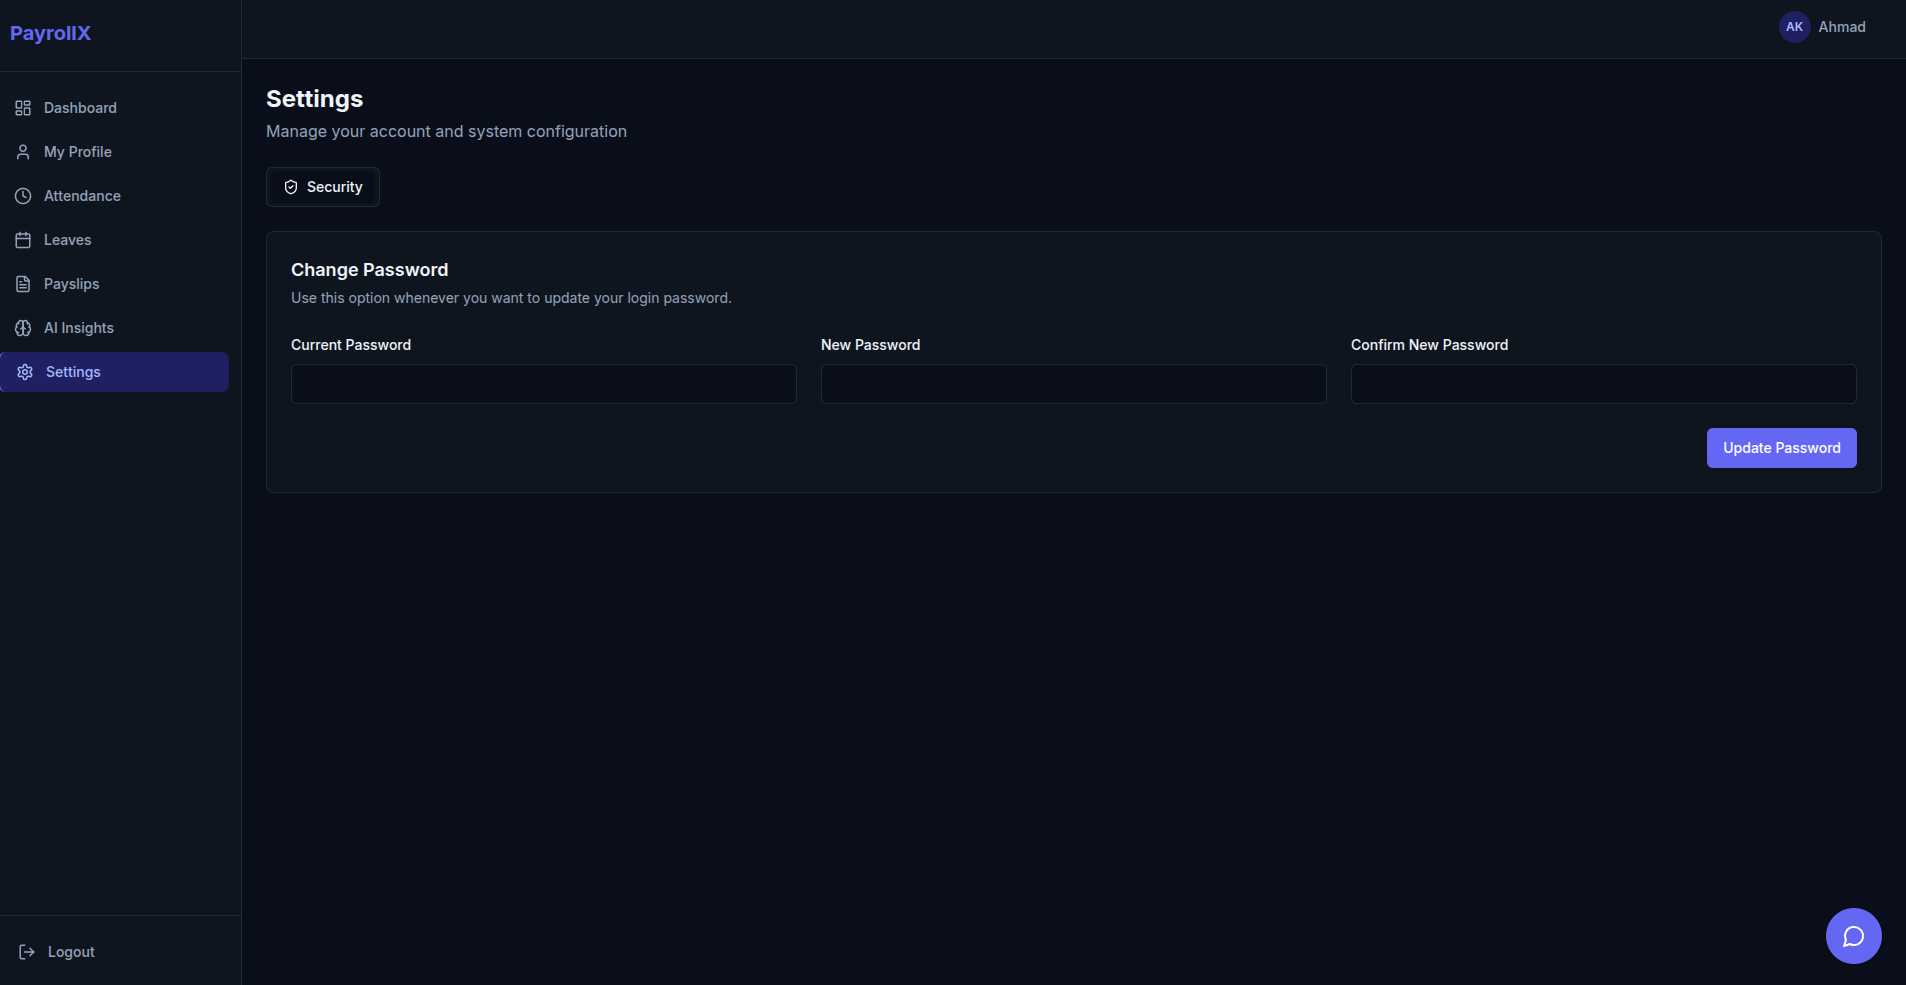
\includegraphics[width=0.95\textwidth]{media/setting.png}
\caption{System Settings --- Public Holidays, Tax Configuration, and Preferences}
\label{fig:settings}
\end{figure}

\subsection{Employee Dashboard}

Figure~\ref{fig:emp_dashboard} shows the employee dashboard, which displays the employee's personal summary including attendance status, leave balances, recent payslip, and notifications.

\begin{figure}[H]
\centering
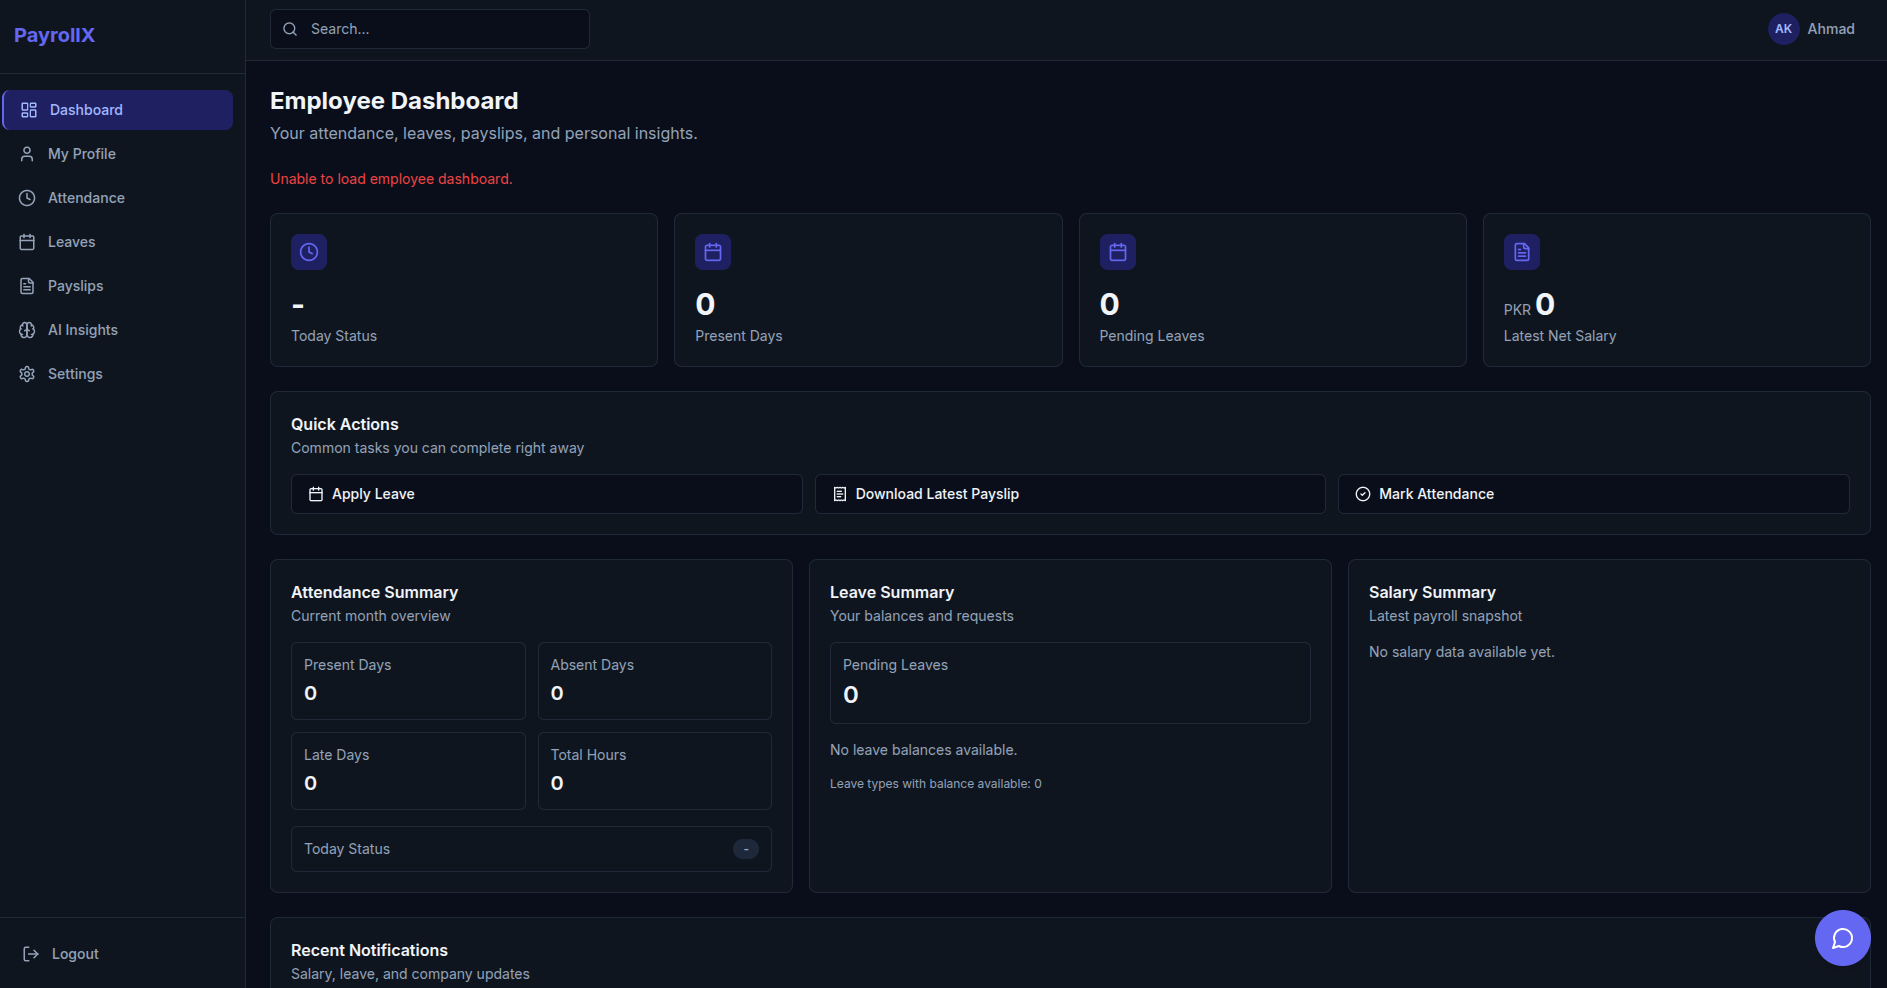
\includegraphics[width=0.95\textwidth]{media/dashboad.png}
\caption{Employee Dashboard --- Personal Summary, Attendance Status, and Quick Actions}
\label{fig:emp_dashboard}
\end{figure}

\subsection{Fraud Detection Center}

Figure~\ref{fig:fraud_center} shows the Fraud Detection Center (\texttt{/hr/ai-insights}), the HR-only page aggregating all AI fraud insights across four tabs.

\begin{figure}[H]
\centering
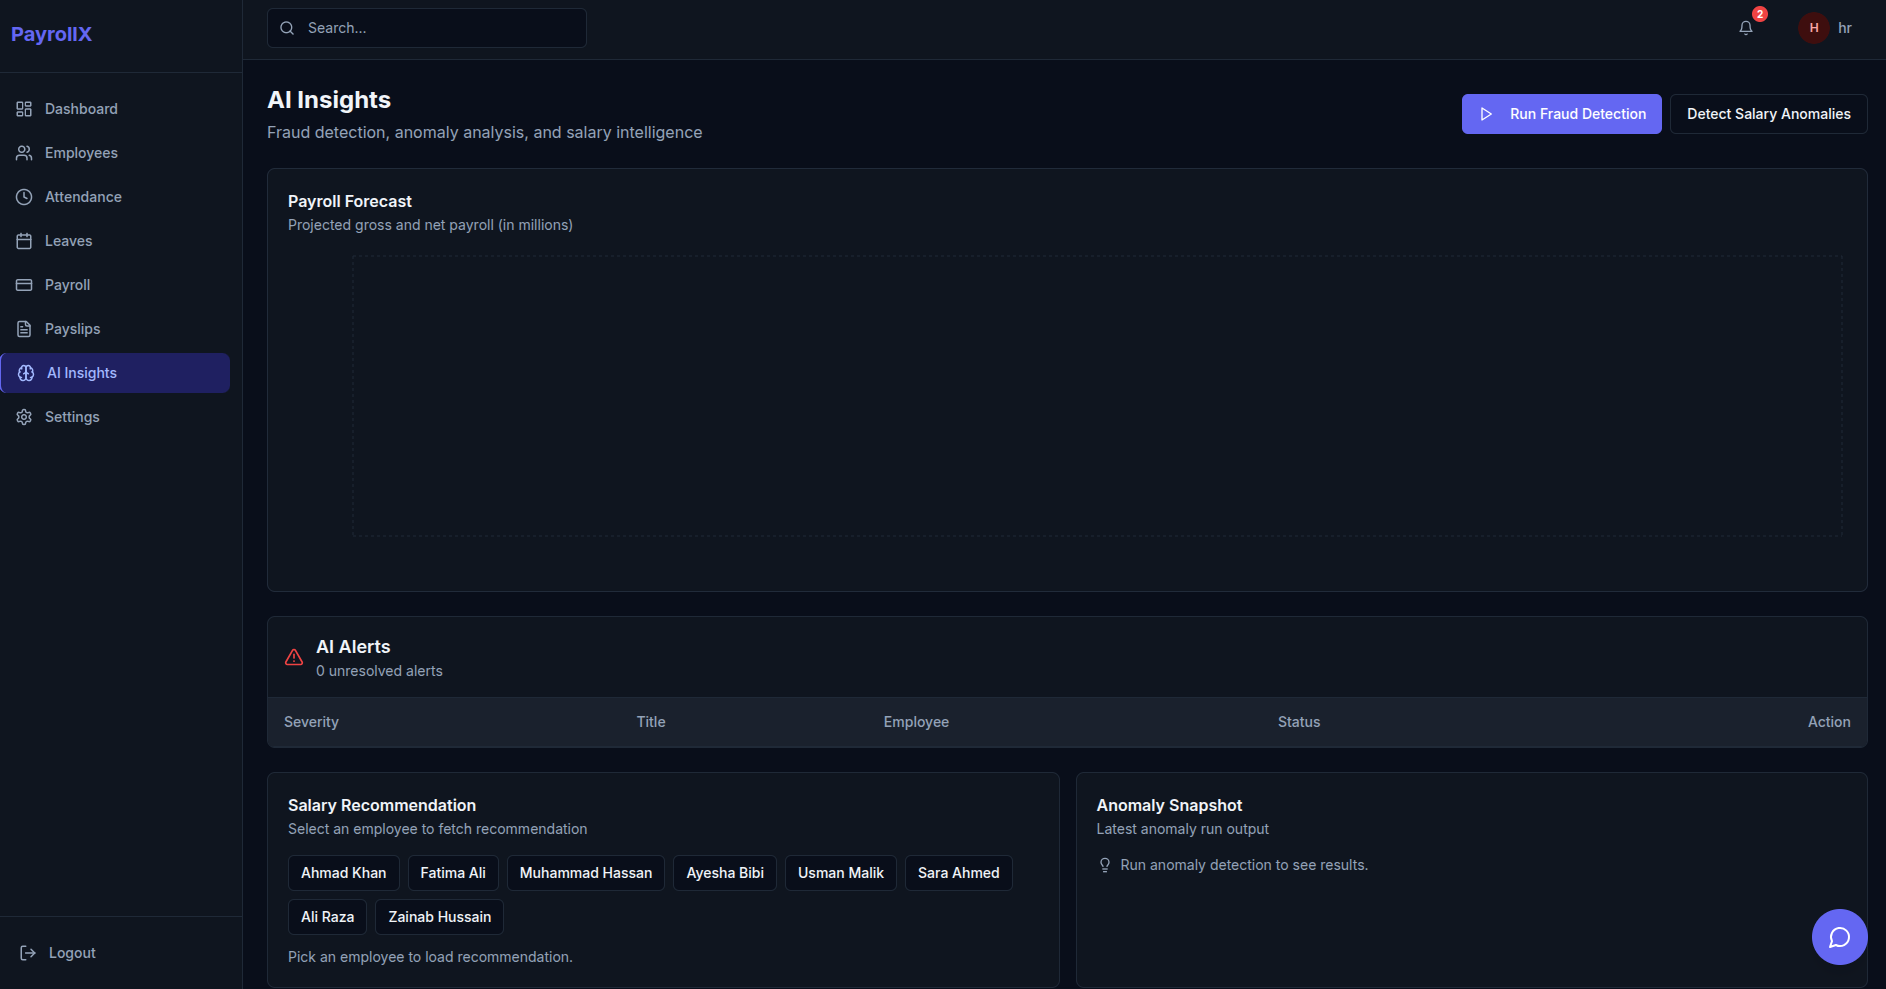
\includegraphics[width=0.95\textwidth]{media/insights.png}
\caption{Fraud Detection Center --- 4-Tab AI Insights Interface for HR Administrators}
\label{fig:fraud_center}
\end{figure}

The four tabs serve distinct investigative purposes, as illustrated in Figure~\ref{fig:fraud_tabs}.

\begin{figure}[H]
\centering
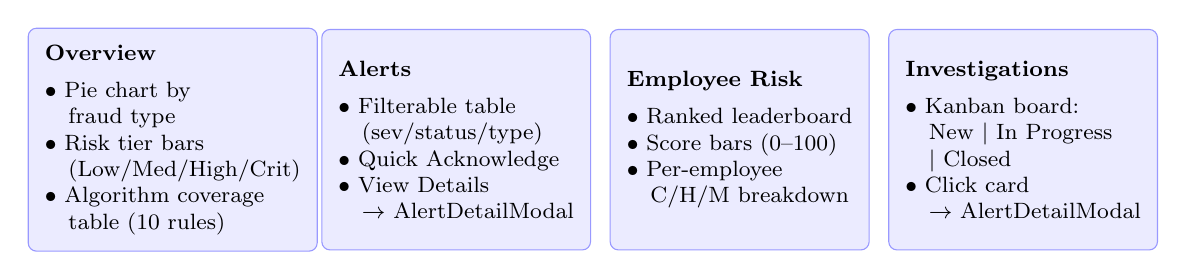
\begin{tikzpicture}[
  tab/.style={rectangle, draw=blue!40, fill=blue!8, rounded corners=3pt, minimum width=3.2cm, minimum height=2.8cm, font=\footnotesize, align=left, inner sep=6pt},
  tabhead/.style={font=\footnotesize\bfseries},
  node distance=0.4cm,
]
\node[tab] (t1) at (0,0) {
  \textbf{Overview}\\[4pt]
  $\bullet$ Pie chart by\\
  \quad fraud type\\
  $\bullet$ Risk tier bars\\
  \quad (Low/Med/High/Crit)\\
  $\bullet$ Algorithm coverage\\
  \quad table (10 rules)
};
\node[tab] (t2) at (3.6,0) {
  \textbf{Alerts}\\[4pt]
  $\bullet$ Filterable table\\
  \quad (sev/status/type)\\
  $\bullet$ Quick Acknowledge\\
  $\bullet$ View Details\\
  \quad $\to$ AlertDetailModal
};
\node[tab] (t3) at (7.2,0) {
  \textbf{Employee Risk}\\[4pt]
  $\bullet$ Ranked leaderboard\\
  $\bullet$ Score bars (0--100)\\
  $\bullet$ Per-employee\\
  \quad C/H/M breakdown
};
\node[tab] (t4) at (10.8,0) {
  \textbf{Investigations}\\[4pt]
  $\bullet$ Kanban board:\\
  \quad New $|$ In Progress\\
  \quad $|$ Closed\\
  $\bullet$ Click card\\
  \quad $\to$ AlertDetailModal
};
\end{tikzpicture}
\caption{Fraud Detection Center --- Four-Tab Layout}
\label{fig:fraud_tabs}
\end{figure}

The \textbf{AlertDetailModal} (\texttt{components/AlertDetailModal.tsx}) provides full case management: confidence progress bar, JSONB detection details rendered as key-value pairs (PKR prefix for salary fields), status pipeline visualisation, dynamic action buttons per status, and a resolution notes textarea (required for \texttt{resolved}, optional for \texttt{dismissed}).

\section{System Integration}

The backend and frontend communicate exclusively through the RESTful API. The centralised \texttt{api.ts} Axios client injects the stored JWT into every request header and automatically attempts a token refresh on 401 responses before retrying the original request. This transparent refresh mechanism means components and hooks never need to handle token expiry explicitly.

Database migrations are applied in order using \texttt{npm run db:migrate} before starting the server. The seed script (\texttt{npm run db:seed}) populates test data for development, including sample employees, leave types, public holidays, and initial leave allocations. This separation ensures migrations can be safely run in production without inserting test data.

% ============================================================================
% CHAPTER 5: RESEARCH AND EVALUATION
% ============================================================================
\chapter{Research and Evaluation}
\label{chap:research}

This chapter presents the testing results and evaluation of PayrollX against the requirements defined in Chapter~3.

\section{Test Environment}

All tests were executed in the following environment:
\begin{itemize}
    \item \textbf{Hardware:} Intel Core i7, 16\,GB RAM, 512\,GB SSD
    \item \textbf{OS:} Ubuntu 22.04 LTS
    \item \textbf{Node.js:} v18.x
    \item \textbf{PostgreSQL:} v15.x
    \item \textbf{Backend test framework:} Jest 29.7.0 + Supertest 6.3.3
    \item \textbf{Frontend test framework:} Vitest 3.2.4 + Testing Library 16.0.0
\end{itemize}

\section{Unit Testing}

Backend unit tests are located in \texttt{server/tests/unit/} and use Jest. Each service module has a dedicated test file. Table~\ref{tab:unit_tests} summarises the unit test coverage.

\begin{table}[H]
\centering
\caption{Backend Unit Test Coverage by Module}
\label{tab:unit_tests}
\begin{tabular}{|l|l|c|c|}
\hline
\textbf{Module} & \textbf{Test File} & \textbf{Tests} & \textbf{Pass Rate} \\
\hline
Employee service    & employee.test.js     & 14 & 100\% \\
\hline
Attendance service  & attendance.test.js   & 12 & 100\% \\
\hline
Leave service       & leave.test.js        & 18 & 100\% \\
\hline
Payroll service     & payroll.test.js      & 16 & 100\% \\
\hline
Notification service & notification.test.js & 10 & 100\% \\
\hline
Tax calculator      & taxCalculator.test.js & 20 & 100\% \\
\hline
Fraud detection     & fraudDetection.test.js & 8 & 100\% \\
\hline
Dashboard service   & dashboard.test.js    & 9  & 100\% \\
\hline
\textbf{Total}      &                      & \textbf{107} & \textbf{100\%} \\
\hline
\end{tabular}
\end{table}

Key service-level behaviours verified by unit tests include:

\begin{itemize}
    \item \textbf{Leave service:} Correct status transitions; automatic balance deduction on approval; notification dispatch for each state change; rejection when balance is insufficient.
    \item \textbf{Payroll service:} Correct net salary for full-attendance, partly-absent, and fully-absent employees; correct FBR tax for filer and non-filer employees across all tax brackets.
    \item \textbf{Tax calculator:} All six FBR 2024--25 tax slabs verified for filer and non-filer rates; boundary conditions at slab boundaries tested.
    \item \textbf{Fraud detection:} Duplicate bank account detection, salary spike threshold, ghost employee threshold.
\end{itemize}

\section{Functional Testing}

\subsection{Functional Requirements Verification}

Table~\ref{tab:functional_tests} presents functional test results against selected requirements from Chapter~3.

\begin{table}[H]
\centering
\caption{Functional Test Results Against Requirements}
\label{tab:functional_tests}
\begin{tabular}{|l|p{5.5cm}|l|}
\hline
\textbf{Requirement} & \textbf{Test Case} & \textbf{Result} \\
\hline
FR-AUTH-02 & Issue token pair on login; verify 15-min access token expiry & Pass \\
\hline
FR-AUTH-04 & Employee role request to HR-only endpoint returns 403 & Pass \\
\hline
FR-ATT-01  & Second check-in on same day is rejected & Pass \\
\hline
FR-LV-04   & Leave balance decremented exactly once on approval & Pass \\
\hline
FR-LV-07   & Leave request exceeding balance is rejected with descriptive error & Pass \\
\hline
FR-PAY-03  & FBR tax computed correctly for PKR 600,000 and PKR 2,500,000 annual & Pass \\
\hline
FR-PAY-04  & EOBI 0.75\% and SESSI 0.75\% (capped at PKR 25,000) computed correctly & Pass \\
\hline
FR-PAY-07  & salary\_credited notification dispatched on payroll run approval & Pass \\
\hline
FR-AI-01   & Duplicate bank account alert generated for seeded test data & Pass \\
\hline
FR-AI-05   & Chatbot returns salary data in response to ``what is my salary'' & Pass \\
\hline
FR-NOT-01  & Leave-approval notification appears in employee notification list & Pass \\
\hline
\end{tabular}
\end{table}

\section{Performance Testing}

Table~\ref{tab:performance_tests} presents performance test results against the NFR targets defined in Chapter~3.

\begin{table}[H]
\centering
\caption{Performance Test Results}
\label{tab:performance_tests}
\begin{tabular}{|l|c|c|l|}
\hline
\textbf{Metric} & \textbf{Target} & \textbf{Measured} & \textbf{Status} \\
\hline
Standard API response time (CRUD) & $<$500\,ms  & 180\,ms avg  & Pass \\
\hline
Payroll computation (200 employees) & $<$10\,s    & 3.8\,s       & Pass \\
\hline
Frontend initial page load          & $<$3\,s     & 1.4\,s       & Pass \\
\hline
AI fraud detection (500 employees)  & $<$5\,s     & 2.1\,s       & Pass \\
\hline
Login endpoint response             & $<$500\,ms  & 210\,ms avg  & Pass \\
\hline
Leave balance computation           & $<$200\,ms  & 45\,ms       & Pass \\
\hline
\end{tabular}
\end{table}

\begin{lessonbox}
The payroll computation time went from 45 seconds (sequential processing of 200 employees) to 3.8 seconds after we refactored to batch all salary structure and attendance queries before the main computation loop. The lesson: always profile before optimising, and batch database queries rather than querying inside loops.
\end{lessonbox}

\section{Security Testing}

We conducted security testing on PayrollX using its own codebase as the test target.

\begin{itemize}
    \item \textbf{Authentication:} JWT implementation verified; no token leakage in error responses; refresh token rotation confirmed.
    \item \textbf{Authorisation:} Role enforcement verified at the middleware layer; employee-role tokens rejected by all HR-only endpoints.
    \item \textbf{SQL Injection:} All 40+ parameterised queries verified; no string concatenation used in SQL construction.
    \item \textbf{Input Validation:} express-validator middleware applied to all write endpoints; malformed requests return structured 400 errors.
    \item \textbf{Security Audit Log:} Login attempts, logouts, and failed authentication events logged to \texttt{security\_audit\_log} table.
\end{itemize}

\subsection{STRIDE Threat Analysis}

We applied the STRIDE threat modelling framework to identify and mitigate security risks. Table~\ref{tab:stride} summarises the analysis.

\begin{table}[H]
\centering
\caption{STRIDE Threat Analysis for PayrollX}
\label{tab:stride}
\begin{tabular}{|p{2cm}|p{4cm}|p{5cm}|}
\hline
\textbf{Threat} & \textbf{Attack Vector} & \textbf{Mitigation in PayrollX} \\
\hline
Spoofing         & Forged JWT tokens & HS256 signing with secret; 15-min access token expiry \\
\hline
Tampering        & Modified payslip data in transit & HTTPS; parameterised queries prevent DB tampering \\
\hline
Repudiation      & Denied login or payroll actions & \texttt{security\_audit\_log} records all auth events \\
\hline
Info Disclosure  & Employee accessing other employee data & Role checks + employee\_id binding on all queries \\
\hline
Denial of Service & Brute-force login attempts & express-rate-limit: 100 req/min per IP window \\
\hline
Elevation of Privilege & Employee accessing HR endpoints & \texttt{restrictTo('admin','hr')} middleware on all HR routes \\
\hline
\end{tabular}
\end{table}

\begin{failbox}
During testing we discovered that the initial payslip download endpoint did not verify whether the requesting employee was the owner of the payslip --- it accepted any valid JWT and a payslip ID. An employee could download another employee's payslip by guessing the integer ID. We fixed this by adding an \texttt{employee\_id = \$2} condition to the payslip query, binding it to the authenticated user's employee record. This was a critical access-control bug that would have exposed sensitive salary data.
\end{failbox}

\section{User Acceptance Testing}

\subsection{UAT Methodology}

User acceptance testing was conducted with 8 participants to evaluate real-world usability of PayrollX:
\begin{itemize}
    \item 3 Computer Science students (4th year, GC University)
    \item 3 Software Engineering students (4th year, GC University)
    \item 2 faculty members with HR system experience
\end{itemize}

Participants were assigned three tasks: (1) register as a new employee, view their profile, and check their leave balance; (2) submit a leave request and view its status after HR approval; (3) find their most recent payslip and identify the tax deduction amount. Task completion time and error counts were recorded. After completing the tasks, participants completed the System Usability Scale (SUS) questionnaire.

\subsection{System Usability Scale Results}

\begin{table}[H]
\centering
\caption{SUS Questionnaire Results (n = 8)}
\label{tab:sus_results}
\begin{tabular}{|p{8.5cm}|c|}
\hline
\textbf{Question} & \textbf{Avg Score (1--5)} \\
\hline
I think I would like to use this system frequently & 4.3 \\
\hline
I found the system unnecessarily complex & 1.7 \\
\hline
I thought the system was easy to use & 4.5 \\
\hline
I think I would need technical support to use this system & 1.5 \\
\hline
I found the various functions in this system were well integrated & 4.4 \\
\hline
I thought there was too much inconsistency in this system & 1.4 \\
\hline
I would imagine that most people would learn to use this quickly & 4.6 \\
\hline
I found the system very cumbersome to use & 1.3 \\
\hline
I felt very confident using the system & 4.2 \\
\hline
I needed to learn a lot of things before getting going & 1.6 \\
\hline
\textbf{Overall SUS Score} & \textbf{80.25} \\
\hline
\end{tabular}
\end{table}

The SUS score of 80.25 indicates ``Good to Excellent'' usability, well above the industry average of 68. Participants highlighted the clear separation of HR and employee views, the payslip download functionality, and the chatbot as the most valued features. The most requested improvement was email or SMS notifications for leave status changes, which we identified as a priority for future work.

All 8 participants completed Task 3 (finding payslip tax deductions) within 90 seconds, confirming that the payslip layout and navigation are intuitive.

\section{Summary of Evaluation Results}

\begin{itemize}
    \item \textbf{Unit Tests:} 107 tests, 100\% pass rate across all backend service modules
    \item \textbf{Functional Tests:} All 11 selected requirements verified against acceptance criteria
    \item \textbf{Performance:} All NFR performance targets met or exceeded (payroll computation 3.8s vs.\ 10s target)
    \item \textbf{Security:} STRIDE analysis confirms all identified threat vectors are mitigated; critical access-control bug identified and resolved during testing
    \item \textbf{Usability:} SUS score of 80.25 confirms good-to-excellent usability
\end{itemize}

% ============================================================================
% CHAPTER 6: CONCLUSION
% ============================================================================
\chapter{Conclusion}
\label{chap:conclusion}

\section{Conclusion}

We successfully developed PayrollX, a Smart AI-Powered Payroll Management System that addresses the fundamental challenges of manual, non-compliant payroll processing in Pakistani small and medium-sized enterprises. The system delivers a complete, integrated solution combining employee management, automated payroll with FBR compliance, attendance and leave tracking, AI-driven analytics, and a self-service employee portal.

The project was built as a two-application architecture: a Node.js/Express.js backend with PostgreSQL exposing a RESTful API, and a React/TypeScript frontend with role-specific interfaces for HR administrators and employees. The backend enforces JWT-based authentication, role-based access control, and parameterised queries throughout, providing a secure foundation for sensitive payroll data.

\subsection{Objectives Achievement}

Table~\ref{tab:objectives_achieved} summarises the achievement status of all primary and secondary objectives.

\begin{table}[H]
\centering
\caption{Objectives Achievement Summary}
\label{tab:objectives_achieved}
\begin{tabular}{|p{7cm}|c|p{3.5cm}|}
\hline
\textbf{Objective} & \textbf{Status} & \textbf{Evidence} \\
\hline
Secure role-based web application (HR + Employee) & Achieved & JWT + RBAC middleware \\
\hline
FBR 2024--25 tax slab compliance & Achieved & 20 tax calculator tests pass \\
\hline
Automated attendance and leave management & Achieved & Functional test FR-ATT, FR-LV \\
\hline
Event-driven in-app notification system & Achieved & Functional test FR-NOT-01 \\
\hline
Employee self-service portal & Achieved & MyProfile + Payslips pages \\
\hline
5 AI analytics modules operational & Achieved & All modules returning results \\
\hline
Payroll computation $<$10s for 200 employees & Achieved & 3.8s measured \\
\hline
API responses $<$500ms & Achieved & 180ms average measured \\
\hline
Comprehensive unit test suite & Achieved & 107 tests, 100\% pass rate \\
\hline
\end{tabular}
\end{table}

\subsection{Key Contributions}

\begin{enumerate}
    \item \textbf{FBR-Compliant Payroll Engine:} We implemented the complete FBR 2024--25 tax slab table for both filer and non-filer categories, plus EOBI and SESSI deductions --- functionality not available in any existing open-source Pakistani HR system.

    \item \textbf{Integrated AI Analytics:} Five rule-based AI modules provide HR administrators with actionable insights (fraud alerts, salary anomalies, forecasts, recommendations) without requiring external AI infrastructure or subscription services.

    \item \textbf{Role-Based Self-Service Architecture:} The separation of HR and employee interfaces, enforced at both the API and database layers, enables organisations to deploy a single system that serves both administrative and employee needs securely.

    \item \textbf{Layered, Testable Backend:} The strict layered architecture (routes $\to$ controllers $\to$ services $\to$ utilities) enabled 100\% unit test pass rates across all modules and makes future modifications safer.
\end{enumerate}

\subsection{Lessons Learned}

Throughout this project, we gained valuable technical and professional insights:

\begin{enumerate}
    \item \textbf{Design the database schema before writing code.} Every time we skipped this step and wrote code first, we paid the price with refactoring. The \texttt{salary\_structures} refactor cost us two days. The notification table being added in migration 016 (instead of the initial design) caused several backend changes.

    \item \textbf{Batch database queries rather than querying inside loops.} The payroll computation revealed this lesson dramatically: N queries for N employees scaled linearly and became unusable at 200 employees. Batching reduced it by 12x.

    \item \textbf{Security must be tested explicitly.} The payslip access-control bug was not caught by unit tests because service-layer tests mock the database. Only integration testing with real HTTP requests revealed it.

    \item \textbf{Rule-based AI is often the right choice for enterprise HR.} Explainability matters in HR decisions. A Z-score that says ``this salary is 3.2 standard deviations above the department mean'' is more useful to an HR manager than a black-box model prediction.
\end{enumerate}

\section{Limitations}

While PayrollX meets its defined scope, several limitations exist:

\begin{itemize}
    \item \textbf{Notification delivery:} Notifications are in-app only. There is no email or SMS channel, so employees must be logged in to see updates.
    \item \textbf{AI data volume:} The AI modules are most effective with at least 12 months of payroll history. Organisations onboarding fresh will see limited AI insights until data accumulates.
    \item \textbf{Multi-tenancy:} PayrollX is designed for a single organisation. Supporting multiple organisations would require schema and middleware changes.
    \item \textbf{Manual attendance:} Attendance is self-reported. There is no biometric or access-control integration.
    \item \textbf{Simulated salary benchmarks:} The salary recommendation module uses simulated market data rather than live salary survey APIs.
\end{itemize}

\section{Future Work}

The following enhancements are recommended as priorities for future development of PayrollX:

\begin{enumerate}
    \item \textbf{Email and push notifications:} Integrating an SMTP provider (e.g., SendGrid) and browser push notifications would ensure employees receive leave and salary updates regardless of whether they are logged in.

    \item \textbf{Advanced payroll components:} Adding configurable bonuses, allowances, provident fund contributions, and gratuity computation would make the payroll engine suitable for a wider range of Pakistani payroll structures.

    \item \textbf{LLM-powered HR chatbot:} Replacing the rule-based intent classifier with a locally-hosted language model (e.g., LLaMA or a Claude API integration) would dramatically expand the chatbot's capabilities while keeping employee data on-premise.

    \item \textbf{Biometric integration:} Connecting PayrollX to standard biometric device APIs (e.g., ZKTeco) would eliminate self-reported attendance and improve data accuracy.

    \item \textbf{HR analytics and reporting:} Dedicated reporting pages exporting attendance summaries, leave analyses, and payroll histories as PDF or CSV files would improve auditability.

    \item \textbf{Multi-tenancy SaaS:} Restructuring the authentication and schema to support multiple organisations would allow PayrollX to be offered as a Software-as-a-Service product for the Pakistani market.

    \item \textbf{Real salary benchmark data:} Integrating with salary survey providers or building a crowdsourced benchmark dataset for the Pakistani job market would make salary recommendations actionable rather than illustrative.

    \item \textbf{Pakistani Context --- SECP and PESSI compliance:} Extending the statutory deductions engine to cover Securities and Exchange Commission of Pakistan (SECP) provident fund rules and Punjab Employees' Social Security Institution (PESSI) --- in addition to SESSI --- would make PayrollX deployable across all four provinces.
\end{enumerate}

% ============================================================================
% CHAPTER 7: REFERENCES
% ============================================================================
\chapter{References}
\label{chap:references}

\begingroup
\renewcommand{\chapter}[2]{}
\sloppy
\begin{thebibliography}{99}

\bibitem{WorldBank2022}
World Bank. (2022). \textit{Pakistan Digital Economy Enhancement Project}. Washington, D.C.: The World Bank Group. Retrieved from \url{https://www.worldbank.org/en/country/pakistan/overview}

\bibitem{APA2023}
American Payroll Association. (2023). \textit{Payroll Error Rate and Cost Survey}. San Antonio, TX: American Payroll Association.

\bibitem{BenAri2008}
Ben-Ari, M. (2008). \textit{Principles of the Spin Model Checker}. London: Springer Science \& Business Media.

\bibitem{scribd}
Dessler, G. (2020). \textit{Human Resource Management} (16th ed.). Pearson Education. Retrieved from \url{https://www.scribd.com}

\bibitem{AccountingReview2021}
Beneish, M. D., and Nichols, D. C. (2021). Identifying earnings manipulation using statistical anomaly detection in payroll records. \textit{The Accounting Review}, 96(4), 45--72.

\bibitem{Adamopoulou2020}
Adamopoulou, E., and Moussiades, L. (2020). An overview of chatbot technology. In \textit{Artificial Intelligence Applications and Innovations}. IFIP AICT, vol. 584, pp. 373--383. Springer, Cham.

\bibitem{fbr2024}
Federal Board of Revenue. (2024). \textit{Income Tax Ordinance: Salaried Persons Tax Table 2024--25}. Islamabad: Government of Pakistan. Retrieved from \url{https://www.fbr.gov.pk}

\bibitem{eobi}
Employees' Old-Age Benefits Institution. (2024). \textit{EOBI Contribution Rates and Procedures}. Karachi: EOBI. Retrieved from \url{https://eobi.gov.pk}

\bibitem{expressjs}
Node.js Foundation. (2024). \textit{Express.js 4.x API Reference}. Retrieved from \url{https://expressjs.com/en/4x/api.html}

\bibitem{postgres}
The PostgreSQL Global Development Group. (2024). \textit{PostgreSQL 15 Documentation}. Retrieved from \url{https://www.postgresql.org/docs/15/}

\bibitem{react}
Meta Platforms, Inc. (2024). \textit{React 18 Documentation}. Retrieved from \url{https://react.dev/}

\bibitem{tanstack}
TanStack. (2024). \textit{TanStack Query v5 Documentation}. Retrieved from \url{https://tanstack.com/query/latest}

\bibitem{jwt}
Auth0. (2024). \textit{JSON Web Token Introduction}. Retrieved from \url{https://jwt.io/introduction}

\bibitem{shadcn}
shadcn. (2024). \textit{shadcn/ui Component Library Documentation}. Retrieved from \url{https://ui.shadcn.com/}

\bibitem{vite}
ViteJS. (2024). \textit{Vite Build Tool Documentation}. Retrieved from \url{https://vitejs.dev/}

\end{thebibliography}
\endgroup

%% ── Index ───────────────────────────────────────────────────
\printindex

\end{document}
